\documentclass[12pt]{article}
\usepackage[pdfborder={0 0 0.5 [3 2]}]{hyperref}%
\usepackage[left=1in,right=1in,top=1in,bottom=1in]{geometry}%
\usepackage[shortalphabetic]{amsrefs}%
\usepackage{amsmath}
\usepackage{enumerate}
% \usepackage{enumitem}
\usepackage{amssymb}                
\usepackage{amsmath}                
\usepackage{amsfonts}
\usepackage{amsthm}
\usepackage{bbm}
\usepackage[table,xcdraw]{xcolor}
\usepackage{tikz}
\usepackage{float}
\usepackage{booktabs}
\usepackage{svg}
\usepackage{mathtools}
\usepackage{cool}
\usepackage{url}
\usepackage{graphicx,epsfig}
\usepackage{makecell}
\usepackage{array}

\def\noi{\noindent}
\def\T{{\mathbb T}}
\def\R{{\mathbb R}}
\def\N{{\mathbb N}}
\def\C{{\mathbb C}}
\def\Z{{\mathbb Z}}
\def\P{{\mathbb P}}
\def\E{{\mathbb E}}
\def\Q{\mathbb{Q}}
\def\ind{{\mathbb I}}

\DeclareMathOperator{\spn}{span}
\DeclareMathOperator{\ran}{ran}

\newtheorem{lemma}{Lemma}
\newtheorem{theorem}{Theorem}
\newtheorem{corollary}{Corollary}
\newtheorem{definition}{Definition}
\newtheorem{assumption}{Assumption}
\newtheorem{hypothesis}{Hypothesis}

\newtheorem{notation}{Notation}

\graphicspath{ {discrete/} }

\begin{document}

We will use Lin's method to prove existence and stability results for multi-pulse on lattices. The model equation here is discrete NLS, but we will do this in a general setting, for which dNLS is a special case. Most of the results for dNLS are already known, at least if we are near the anti-continuum limit (see, for example, Pelinovsky and Kevrekidis, 2005). The idea is that if we can find an appropriate generalization and setup for Lin's method, we can check it on dNLS. 

\section{Setup and Main Theorems}

\subsection{Background}

Consider the lattice PDE on $\R^s$
\begin{equation}\label{latticePDE}
\dot{u}_n = f(u_n)
\end{equation}
where $f$ is a smooth nonlinear operator which involves involves a finite number (greater than 1) of indices near $n$. We will make one of the following two assumptions regarding symmetry of equation \eqref{latticePDE}.

\begin{hypothesis}\label{symmetryhyp}
There exists a group $G$ for which the group action is unitary group of symmetries $t(\theta)$ on $\R^s$ such that $f(t(\theta)u) = t(\theta)f(u)$ for all $\theta \in G$ and all $u \in \R^s$. For the group $G$, we have one of the following:
\begin{enumerate}[(i)]
\item $G$ is a finite group.
\item $G = (\R, +)$.
\end{enumerate}
\end{hypothesis}

An equilibrium solution satisfies the stationary equation 
\begin{equation}\label{stationaryeq}
f(u_n) = 0
\end{equation}
We can rewrite the stationary equation as a system of first-order difference equations of the form
\begin{equation}\label{diffeq}
U(n+1) = F(U(n))
\end{equation}
where $U \in \R^d$ and $F:\R^d \rightarrow \R^d$ for some $d > 1$ which depends on how many indices near $n$ are used by $f$. Since $f$ is smooth, $F$ is smooth as well. The group $G$ also induces  a group action on $\R^d$; this action is a unitary group of symmetries $T(\theta)$ on $\R^d$ such that $F(T(\theta)U) = T(\theta)F(U)$ for all $\theta \in G$ and all $U \in \R^d$. We take the following hypothesis regarding $F$.

\begin{hypothesis}\label{initialhyp}
We assume the following regarding \eqref{diffeq}.
\begin{enumerate}[(i)]
\item 0 is a hyperbolic equilibrium for $F$, i.e. $F(0) = 0$ and $DF(0)$ has no eigenvalues on the unit circle. Thus we can find a radius $r > 1$ such that for all eigenvalues $\nu$ of $DF(0)$ we have $|\nu| \leq 1/r$ or $|\nu| > r$.
\item $\dim E^s, \dim E^u \geq 1$, where $E^s$ and $E^u$ are the stable and unstable eigenspaces of $DF(0)$.
\item There exists a symmetric homoclinic orbit (primary pulse) solution $Q(n)$ to \eqref{diffeq} which connects the equilibrium at 0 to itself.
\end{enumerate}
\end{hypothesis}

Finally, we will take the following hypothesis regarding the intersection of the stable manifold $W^s(0)$ and unstable manifold $W^u(0)$. The form of this hypothesis depends on which symmetry hypothesis we choose.

\begin{hypothesis}\label{intersectionhyp}
If Hypothesis \ref{symmetryhyp}(i) holds, then the stable and unstable manifolds $W^s(0)$ and $W^u(0)$ intersect transversely.

If Hypothesis \ref{symmetryhyp}(ii) holds, then the tangent spaces of the stable and unstable manifolds $W^s(0)$ and $W^u(0)$ have a one-dimensional intersection at $Q(n)$ given by $S_1(n) = S Q(n)$, where $S$ is the infinitesimal generator of $T(\theta)$.
\end{hypothesis}

If follows from the symmetry relation $F(T(\theta)u) = T(\theta)F(u)$ that $U(n)$ is a solution to \eqref{diffeq} if and only if $T(\theta)U(n)$ is also a solution. We note that for Hypothesis \ref{intersectionhyp}(i), the group $G$ can be the trivial group consisting only of the identity.

\subsection{Existence Problem}
First, we will prove the existence of multi-pulse solutions to \eqref{latticePDE}. These are solutions that resemble multiple, well-separated copies of the primary pulse $Q(n)$.

Choose an integer $m > 1$ (the number of pulses), and let $N_i$ ($i = 1, \dots, m-1$) be the desired distances (in lattice points) between the $m$ copies of $Q(n)$. Let 
\begin{equation}\label{Nipm}
\begin{aligned}
N_i^+ &= \lfloor \frac{N_i}{2} \rfloor \\
N_i^- &= N_i - N_i^+
\end{aligned}
\end{equation}
and note that either $N_i^+ = N_i^-$ (if $N_i$ is even) or $N_i^+ = N_i^- - 1$ (if $N_i$ is odd). Let $N = \min\{ N_i^\pm \}$. In addition, let $N_0^- = -\infty$ and $N_m^+ = \infty$. We will look for a solution which is a piecewise perturbation of $n$ consecutive copies of $Q(n)$. This is a solution of the form
\begin{align}\label{Upiecewise}
U_i^-(n) &= T(\theta_i) Q(n) + W_i^-(n) && n \in [-N_{i-1}^-, 0] \\
U_i^+(n) &= T(\theta_i) Q(n) + W_i^+(n) && n \in [0, N_i^+]
\end{align}
where $\theta_i = G$ and the pieces are joined together end-to-end as in San98.

In addition to satisfying \eqref{diffeq}, we require that the pieces $U_i^\pm(n)$ match at the interval endpoints. Thus $U_i^\pm(n)$ must satisfy the system of equations
\begin{equation}\label{Usystem}
\begin{aligned}
(U_i^\pm)(n+1) &= F(U_i^\pm(n))  \\
U_i^+(N_i^+) - U_{i+1}^-(-N_i^-) &= 0 \\
U_i^+(0) - U_i^-(0) &= 0
\end{aligned}
\end{equation}
for $i = 1, \dots, m$. Expanding $F$ in a Taylor series about $T(\theta_i) Q(n)$, we get
\begin{align*}
F(U_i^\pm(n)) &= F(T(\theta_i) Q(n) + W_i^\pm(n)) \\
&= F(T(\theta_i) Q(n)) + DF_{U}(T(\theta_i) Q(n)) W_i^\pm + G(W_i^\pm(n)) \\
&= A(n; \theta_i) W_i^\pm + G(W_i^\pm(n))
\end{align*}
where
\begin{align*}
A(n; \theta_i) &= DF(T(\theta_i) Q(n))\\
G(W_i^\pm(n)) &= \mathcal{O}(|W_i^\pm|^2)
\end{align*}
with $G(0) = 0$ and $DG(0) = 0$. Finally, let 
\begin{equation}\label{defdi}
d_i = T(\theta_{i+1}) Q(-N_i^-) - T(\theta_i) Q(N_i^+)
\end{equation}

Substituting these into \eqref{Usystem}, we obtain the following system of equations for the piecewise function $W_i^\pm$.
\begin{align}
W_i^\pm(n+1) &= A(n; \theta_i) W_i^\pm + G(W_i^\pm(n)) \label{Wsystem1} \\
W_i^+(N_i^+) - W_{i+1}^-(-N_i^-) &= d_i \label{Wsystem2} \\
W_i^+(0) - W_i^-(0) &= 0 \label{Wsystem3}
\end{align}

The variational and adjoint variational equations associated with \eqref{diffeq} come from the linearization of \eqref{diffeq} about the primary pulse solution $Q(n)$.
\begin{align}
V(n+1) &= A(n; 0) V(n) \label{vareq} \\
Z(n+1) &= [A(n; 0)^*]^{-1} Z(n) \label{adjvareq} 
\end{align}
where $A(n; 0) = D_U F(Q(n))$. If we take Hypothesis \ref{symmetryhyp}(i), the variational equation does not have a bounded solution, and we have the decomposition $\R^d = Y^+ \oplus Y^-$, where $Y^+ = T_{Q(0)} W^s(0)$ and $Y^- = T_{Q(0)} W^u(0)$. Since $T(\theta)$ is unitary, we also have the decomposition $\R^d = T(\theta_i) Y^+ \oplus T(\theta_i) Y^-$.

If we instead take Hypothesis \ref{symmetryhyp}(ii), the variational equation \eqref{vareq} has a bounded solution $S_1(n)$. To see this, recall that $S_1(n) = S Q(n)$, where $S$ is the infinitesimal generator for the symmetry group $T(\theta)$. $S$ is defined by
\begin{equation}
S = \frac{d}{d \theta} T(\theta)\Big|_{\theta = 0}
\end{equation}
Differentiating $T(\theta) Q(n+1) = F(T(\theta)Q(n))$ with respect to $\theta$, we have
\[
\frac{d}{d \theta}T(\theta) Q(n+1) = F(T(\theta)Q(n)) \frac{d}{d \theta}T(\theta) Q(n)
\]
Taking $\theta = 0$, since $F$ is smooth and $T(0) = I$, this becomes $S Q(n+1) = DF(Q(n) S Q(n)$, from which we conclude that $S_1(n)$ is a solution to the variational equation. 

From Hypothesis \ref{intersectionhyp}, the variational equation \eqref{vareq} has no other linearly independent bounded solution. Thus we can decompose the tangent spaces $W^s(0)$ and $W^u(0)$ at $Q(0)$ as
\begin{align*}
T_{Q(0)} W^u(0) &= Y^- \oplus \R S_1(0) \\
T_{Q(0)} W^s(0) &= Y^+ \oplus \R S_1(0)
\end{align*}
It also follows from Hypothesis \ref{intersectionhyp} that the adjoint variational equation \eqref{adjvareq} has a unique bounded solution $Z_1(n)$. By Lemma \ref{evolop} below, $Z_1(0) \perp S_1(0) \oplus Y^- \oplus Y^+$, thus we can decompose $\R^d$ as
\begin{equation}\label{nontdecomp}
\R^d = \R S_1(0) \oplus Y^+ \oplus Y^- \oplus \R Z_1(0)
\end{equation}
Since $T(\theta)$ is unitary, we also have the decomposition
\begin{equation}\label{nontdecompT}
\R^d = \R T(\theta_i) S_1(0) \oplus T(\theta_i) Y^+ \oplus T(\theta_i) Y^- \oplus \R T(\theta_i) Z_1(0)
\end{equation}

If Hypothesis \ref{symmetryhyp}(ii) holds, we may without loss of generality choose $W_i^\pm$ so that 
\begin{equation}\label{W0loc}
W_i^\pm(0) \in T(\theta_i) Y^+ \oplus T(\theta_i) Y^- \oplus \R T(\theta_i) Z_1(0)
\end{equation}
since the parameter $\theta_i$ in \eqref{Upiecewise} takes care of the direction $T(\theta_i) S_1(0)$ along the symmetry.

We have the following theorems regarding existence of multi-pulse solution to \eqref{diffeq}. Proofs will follow in a later section. First, if Hypothesis \ref{symmetryhyp}(i) holds, we have a unique $m-$pulse solution to \eqref{diffeq}.

\begin{theorem}\label{transversemulti}
Consider the difference equation
\begin{equation}\label{diffeqm1}
U(n+1) = F(u(n))
\end{equation}
where $U \in R^d$ for $d > 1$. Assume Hypotheses \ref{symmetryhyp}(i), \ref{initialhyp}, and \ref{intersectionhyp}. Let $Q(n)$ be the primary pulse solution to \eqref{diffeqm1}. Choose $m > 1$ and positive integers $N_1, \dots, N_{m-1}$, and define $N_i^\pm$ as in \eqref{Nipm}. Choose any $\theta_1, \dots, \theta_m \in G$. Then, for sufficiently large $N$, where $N = \min\{ N_i^\pm : i = 1, \dots, m-1 \}$, there exists a unique $m-$pulse solution $Q_m(n)$ to \eqref{diffeqm1} which can be written piecewise as 
\begin{align}
U_i^-(n) &= T(\theta_i) Q(n) + W_i^-(n) && n \in [-N_{i-1}^-, 0] \\
U_i^+(n) &= T(\theta_i) Q(n) + W_i^+(n) && n \in [0, N_i^+]
\end{align}
where $N_0 = N_m = \infty$. For the remainder terms $W_i^\pm(n)$ we have the following estimates
\begin{equation}\label{Westimates}
\begin{aligned}
||W_i^\pm|| &\leq C r^{-N} \\
W_i^+(N_i^+) &= T(\theta_{i+1}) Q(-N_i^-) + \mathcal{O}(r^{-2N}) \\
W_{i+1}^-(-N_i^-) &= T(\theta_i) Q(N_i^+) + \mathcal{O}(r^{-2N})
\end{aligned}
\end{equation}
\end{theorem}

If \ref{symmetryhyp}(ii) holds, we will not in general have solution to \eqref{diffeq}, since Lin's method generically yields a solution with $m$ jumps in the direction of $Z_1(0)$. We can, however, prove a criterion for such a solution to exist, which amounts to solving $m$ jump conditions.

\begin{theorem}\label{ntmulti}
Consider the difference equation
\begin{equation}\label{diffeqm2}
U(n+1) = F(u(n))
\end{equation}
where $U \in R^d$ for $d > 1$. Assume Hypotheses \ref{symmetryhyp}(ii), \ref{initialhyp}, and \ref{intersectionhyp} Let $Q(n)$ be the primary pulse solution to \eqref{diffeqm2}. Choose $m > 1$ and positive integers $N_1, \dots, N_{m-1}$, and define $N_i^\pm$ as in \eqref{Nipm}. Let $\theta_1, \dots, \theta_m \in \R$. Then, for sufficiently large $N$, where $N = \min\{ N_i^\pm : i = 1, \dots, m-1 \}$, there exists a unique $m-$pulse solution $Q_m(n)$ to \eqref{diffeqm2} of the form
\begin{align}
U_i^-(n) &= T(\theta_i) Q(n) + W_i^-(n) && n \in [-N_{i-1}^-, 0] \\
U_i^+(n) &= T(\theta_i) Q(n) + W_i^+(n) && n \in [0, N_i^+]
\end{align}
if and only if the following $m$ jump conditions 
\begin{align*}
\xi_i &= 0 && i = 1, \dots, m
\end{align*}
are satisfied, where
\begin{equation}\label{jumpZ}
\begin{aligned}
\xi_1 &= \langle T(\theta_1) Z_1(N_1^+), T(\theta_2) Q(-N_1^-) \rangle + R_1  \\
\xi_i &= \langle T(\theta_i) Z_1(N_i^+), T(\theta_{i+1}) Q(-N_i^-) \rangle
- \langle T(\theta_i) Z_1(-N_{i-1}^-), T(\theta_{i-1}) Q(N_{i-1}^+) + R_i &&
i = 2, \dots, m-1 \\
\xi_m &= -\langle T(\theta_m) Z_1(-N_{m-1}^-), T(\theta_{m-1}) Q(N_{m-1}^+) + R_m
\end{aligned}
\end{equation}
and the remainder terms have uniform bound
\[
|R_i| \leq C r^{-3N}
\]
The estimates \eqref{Westimates} on $W_i^\pm$ from Theorem \ref{transversemulti} hold in this case.
\end{theorem}

\subsection{Stability Problem}

Now that we have proven existence of multi-pulse solutions to \eqref{diffeq}, we will look at their spectral stability. For this, we assume Hypotheses \ref{symmetryhyp}(ii), \ref{initialhyp}, \ref{intersectionhyp} from the previous section. Let $Q_m(n)$ be an $m-$pulse solution to \eqref{diffeq}, constructed as in the previous section, and write $Q_m(n)$ piecewise as
\begin{align}\label{qmpiecewise}
Q_m(n) =
\begin{cases}
T(\theta_i) Q(n) + \tilde{Q}_i^-(n) & n = [-N_{i-1}^-, 0] \\
T(\theta_i) Q(n) + \tilde{Q}_i^+(n) & n = [0, N_i^+] \\
\end{cases}
\end{align}
where $\theta_i \in \R$ and the interval endpoints $N_i^\pm$ are defined in \eqref{Nipm}, with $N_0^- = -\infty$ and $N_m^+ = \infty$. From $Q_m(n)$, we can obtain an equilibrium solution $q_m(n) \in \R^s$ to \eqref{latticePDE}. 

To obtain the eigenvalue problem associated with \eqref{latticePDE}, we substitute the standard linearization ansatz $u(n) = q_m(n) + \epsilon v(n) e^{\lambda t}$ and keep terms up to order $\epsilon$. This gives us the eigenvalue problem
\begin{equation}\label{EVP}
Df(q_m(n))v(n) = \lambda v(n)
\end{equation}
As we did in the previous section with the stationary equation \eqref{stationaryeq}, we write \eqref{EVP} as a system of first-order difference equations. Using the same procedure to do this as in the previous section, we obtain the eigenvalue problem in $\R^d$
\begin{align}\label{latticeEVP}
V(n+1) = DF(Q_m(n)) V(n) + \lambda B V(n)
\end{align}
where $F: \R^d \rightarrow \R^d$ is the same as in equation \eqref{diffeq} and $B$ is a bounded, $d\times d$ constant-coefficient matrix. We make the following hypothesis regarding $B$ and $T(\theta)$, which holds in most applications.
\begin{hypothesis}\label{BTcommutehyp}
For all $\theta \in G$, $T(\theta) B = B T(\theta)$.
\end{hypothesis}
Since $Q_m(n)$ decays exponentially to 0, $DF(Q_m(n))$ is exponentially asymptotic to the constant coefficient matrix $DF(0)$, which is hyperbolic by Hypothesis \ref{initialhyp}. 

We will also assume one of the following Melnikov-like conditions.
\begin{hypothesis}\label{melnikovhyp}
One of the following Melnikov conditions holds.
\begin{enumerate}[(i)]
\item
\[
M_1 = \sum_{n=-\infty}^\infty \langle Z_1(n+1), B S_1(n) \rangle \neq 0
\]
\item 
\[
M_1 = \sum_{n=-\infty}^\infty \langle Z_1(n+1), B S_1(n) \rangle = 0
\]
By the Fredholm alternative, there exists $T_1(n)$ such that 
\[
T_1(n+1) = DF(Q(n)) T_1(n) + B S_1(n)
\]
We assume that the higher order Melnikov sum is nonzero.
\[
M_2 = \sum_{n=-\infty}^\infty \langle Z_1(n+1), B T_1(n) \rangle \neq 0 
\]
In addition, we assume that $T_1(n)$ is exponentially localized. (We might be able to show this.)
\end{enumerate}
\end{hypothesis}

We can now state the stability theorem, in which we locate the eigenvalues of \eqref{latticePDE}.

\begin{theorem}\label{stabilitytheorem}
Assume Hypotheses \ref{symmetryhyp}(ii), \ref{initialhyp}, \ref{intersectionhyp}, and \ref{BTcommutehyp}. Let $Q_m(n)$ be discrete $m-$pulse equilibrium solution to \eqref{latticePDE}, constructed according to Theorem \ref{ntmulti}. Then there exists a bounded, nonzero solution $V(n)$ of the eigenvalue problem \eqref{latticeEVP} for $|\lambda| < \delta$ if and only if $\det E(\lambda) = 0$, where
\begin{equation}\label{Elambda}
E(\lambda) = \begin{cases}
\det(A - M_1 \lambda I + R(\lambda))
& \text{Hypothesis \ref{melnikovhyp}(i) holds} \\
\det(A - M_2 \lambda^2 I + R(\lambda))
& \text{Hypothesis \ref{melnikovhyp}(ii) holds}
\end{cases}
\end{equation}
$M_1$ and $M_2$ are defined in Hypothesis \eqref{melnikovhyp}. The matrix $A$ is tridiagonal and is given by
\begin{align}\label{matrixA}
A &= \begin{pmatrix}
-a_1 & a_1 & & &  \\
-\tilde{a}_1 & \tilde{a}_1 - a_2 & a_2 \\
& -\tilde{a}_2 & \tilde{a}_2 - a_3 & a_3 \\
& \ddots & & \ddots \\
& & & -\tilde{a}_{m-1} & \tilde{a}_{m-1}  \\
\end{pmatrix}
\end{align}
where
\begin{align*}
a_i &= \langle T(\theta_i) Z_1(N_i^+), T(\theta_{i+1}) S_1(-N_i^-) \rangle \\
\tilde{a}_i &= \langle T(\theta_{i+1}) Z_1(-N_i^-), T(\theta_i) S_1(N_i^+) \rangle
\end{align*}
and the remainder term has bound
\begin{align}\label{Rbound2}
|R(\lambda)| \leq C\left( (r^N + |\lambda|)^3 \right)
\end{align}
\end{theorem}

\section{Discrete NLS}

\subsection{Background}

We will apply the results of the previous section to the discrete NLS equation (dNLS). The normalized form of dNLS is
\begin{equation}\label{dNLS}
i\dot{u}_n + \epsilon(u_{n+1} - 2 u_n + u_{n-1}) + |u_n|^2 u_n = 0
\end{equation}
The parameter $\epsilon$ represents the coupling between nodes. Equation \eqref{dNLS} is Hamiltonian (Kev09x), with energy $H$ given by
\[
H = -\sum_{n=-\infty}^\infty\left( \epsilon|u_n - u_{n-1}|^2
-\frac{1}{2}|u_n|^4 \right)
\]

We are interested in stationary solutions in a ``co-rotating'' frame, which are solutions of the form $\phi_n e^{i \omega t}$. To that end, we make the substitution $u_n \mapsto u_n e^{i \omega t}$ in \eqref{dNLS} and simplify to get
\begin{equation}\label{dNLSrot}
i\dot{u}_n + \epsilon(u_{n+1} - 2 u_n + u_{n-1}) - \omega u_n + |u_n|^2 u_n = 0
\end{equation}

Equilibrium solutions satisfy
\begin{equation}\label{dNLSequilib}
\epsilon(u_{n+1} - 2 u_n + u_{n-1}) - \omega u_n + |u_n|^2 u_n = 0
\end{equation}
The anti-continuum limit occurs at $\epsilon = 0$, at which point \eqref{dNLSequilib} becomes an algebraic equation. Any function $u(n)$ with $u(n) \in \{ 0, \pm \sqrt{\omega}\}$ is a solution to \eqref{dNLSequilib} when $\epsilon = 0$. We are interested in what happens as $\epsilon$ increases.

The dNLS equation possesses two real-valued, symmetric, single pulse solutions (up to rotation): on-site solutions, which are centered on a single lattice point; and off-site solutions, which are centered between two adjacent lattice points (Kev09x). The on-site solution has a single eigenvalue at 0 from the rotational symmetry. The off-site solution has in addition a pair of real eigenvalues; since the off-site solution is spectrally unstable, we will only consider the on-site solution from here on. 

Let $q(n)$ be the on-site solution. I believe this exists for all $\epsilon$, as it exists in both the anti-continuum limit and the continuum limit; this should be somewhere in Chapter 2 of Kev09x.

\subsection{Real-valued multi-pulses}

We will now show existence of multi-pulse solutions. These resemble multiple, well-separated copies of the on-site, primary pulse solution $q(n)$. An argument using the implicit function theorem shows that these solutions exist near the anti-continuum limit [Reference]. We will use Lin's method to give an existence proof which relies on the pulse separation instead of proximity to the anti-continuum limit.

First, we will look for real-valued solutions to \eqref{dNLSequilib}. In this case, the stationary equation reduces to
\begin{equation}\label{dNLSequilibreal}
\epsilon(u_{n+1} - 2 u_n + u_{n-1}) - \omega u_n + u_n^3 = 0
\end{equation}
The symmetry group is $G = (\{1, -1\}, \cdot)$, and the group action on $l^\infty(\Z)$ is $g(\theta) = \theta$, i.e. multiplication by $\theta$. Thus Hypothesis \eqref{symmetryhyp}(i) is satisfied.

To write this as a first order system, let $\tilde{u}_n = u_{n-1}$. Then for $\epsilon > 0$, \eqref{dNLSequilibreal} is equivalent to the difference equation in $\R^2$
\begin{equation}\label{dnlsdiffR2}
\begin{pmatrix}
u \\ \tilde{u}
\end{pmatrix}_{n+1} =
\begin{pmatrix}
\frac{\omega}{\epsilon} + 2 & -1 \\
1 & 0
\end{pmatrix}
\begin{pmatrix}
u \\ \tilde{u}
\end{pmatrix}_n
- \frac{1}{\epsilon} 
\begin{pmatrix}
u_n^3 \\ 0
\end{pmatrix}
\end{equation}
where we have separated the RHS into linear and nonlinear parts. This is of the form of equation \eqref{diffeq}, where $U = (u, \tilde{u})$ and we have written $F: \R^2 \rightarrow \R^2$ as $F(U) = DF(0) U + G(U)$. The symmetry group $G$ acts on $\R^2$ via $T(\theta) = \theta I$. The rest state $U(n) = 0$ is an equilibrium solution. For $\epsilon, \omega > 0$, $DF(0)$ has a pair of real eigenvalues $\{r, 1/r \}$, where $r$ depends on both $\epsilon$ and $\omega$, and is given by
\begin{align}\label{defr}
r = 1 + \frac{\omega}{2 \epsilon} \left( 1 + \sqrt{1 + \frac{4 \epsilon}{\omega}} \right) > 1
\end{align}
As $\epsilon \rightarrow \infty$, $r \rightarrow 1$, thus the spectral gap decreases with increasing $\epsilon$. As $\epsilon \rightarrow 0$, $r \rightarrow \infty$.

It follows that 0 is a hyperbolic equilibrium point with 1-dimensional stable and unstable manifolds. Thus Hypothesis \ref{initialhyp} is satisfied, where the existence of a primary pulse solution was discussed above. Since the variational equation does not have a bounded solution, the stable and unstable manifolds intersect transversely, thus Hypothesis \ref{intersectionhyp} is satisfied. 

Using Theorem \ref{transversemulti}, for sufficiently large $N$ (which depends on $r$, thus $\omega$ and $\epsilon$) there exist $m-$pulse solutions of the form
\begin{align*}
Q_i^-(n) &= \theta_i Q(n) + W_i^-(n) && n \in [-N_{i-1}^-, 0] \\
Q_i^+(n) &= \theta_i Q(n) + W_i^+(n) && n \in [0, N_i^+]
\end{align*}
for any choices $\theta_i = \pm 1$ and lengths $N_i \geq N$. 

\subsection{No other multi-pulses}

We will now show that (up to rotation), there are no other multi-pulse soliton solutions to dNLS. In particular, there are no multi-pulse solutions with phase differences other than $0$ and $\pi$. For convenience, we will reuse much of the notation from the previous section. 

Since we are now considering complex-valued solutions to \eqref{dNLSequilib}, the symmetry group is $G = (\R, +)$, and the group action on $l^\infty(\C)$ is $g(\theta)u(n) = e^{i \theta}u(n)$, i.e. rotation by $\theta$. Thus Hypothesis \ref{symmetryhyp}(ii) is satisfied.

Next, we write dNLS as a two-dimensional system in real variables. Substituting $u = v + i w$ into equation \eqref{dNLSrot} and equating real and imaginary parts, we obtain the equivalent equation
\begin{equation}\label{dNLSreal}
\begin{aligned}
\dot{v}_n  &+ \epsilon (w_{n+1} - 2 w_n + w_{n-1}) - \omega w_n + v_n^2 w_n + w_n^3 = 0 \\
-\dot{w}_n &+ \epsilon (v_{n+1} - 2 v_n + v_{n-1}) - \omega v_n + v_n w_n^2 + v_n^3 = 0
\end{aligned}
\end{equation}
where $v, w \in l^\infty(\R)$. 

Let $\tilde{v}_n = v_{n-1}$ and $\tilde{w}_n = w_{n-1}$. Then stationary solutions to \eqref{dNLSreal} satisfy the difference equation 
\begin{equation}\label{dnlsdiffR4}
U(n+1) = F(U(n))
\end{equation}
in $\R^4$, where $U(n) = (v(n), \tilde{v}(n), w(n), \tilde{w}(n))$ and $F:\R^4 \rightarrow \R^4$ is defined by
\begin{equation}\label{FdNLS}
F\begin{pmatrix}
v \\ \tilde{v} \\ w \\ \tilde{w}
\end{pmatrix} =
\begin{pmatrix}
\frac{\omega}{\epsilon} + 2 & -1 & 0 & 0 \\
1 & 0 & 0 & 0 \\
0 & 0 & \frac{\omega}{\epsilon} + 2 & -1 \\
0 & 0 & 1 & 0
\end{pmatrix}
\begin{pmatrix}
v \\ \tilde{v} \\ w \\ \tilde{w}
\end{pmatrix}
- \frac{1}{\epsilon} 
\begin{pmatrix}
v w^2 + v^3 \\ 0 \\ v^2 w + w^3 \\ 0
\end{pmatrix}
\end{equation}
We have again separated the RHS into linear and nonlinear parts, so that the RHS is of the for $F(U) = DF(0) U + G(U)$. The rest state $U(n) = 0$ is an equilibrium solution. The symmetry group $G$ acts on $\R^4$ via $T(\theta)$, where
\begin{align}\label{TdNLS}
T(\theta) =
\begin{pmatrix}
\cos\theta & 0 &-\sin\theta & 0 \\
0 & \cos\theta & 0 &-\sin\theta \\
\sin\theta & 0 & \cos\theta & 0 \\
0 & \sin\theta & 0 & \cos\theta 
\end{pmatrix}
\end{align}
$T(\theta)$ has infinitesimal generator $S$, which is given by
\begin{align}\label{dnlsSgen}
S =
\begin{pmatrix}
0 & 0 &-1 & 0 \\
0 & 0 & 0 &-1 \\
1 & 0 & 0 & 0 \\
0 & 1 & 0 & 0 
\end{pmatrix}
\end{align}

For $\epsilon, \omega > 0$, $DF(0)$ has eigenvalues $\{r, 1/r\}$, each of which has multiplicity 2, since $DF(0)$ is block diagonal with two identical blocks; the constant $r$ is the same as in the previous section, and is defined in equation \eqref{defr}. Thus $DF(0)$ is hyperbolic with 2-dimensional stable and unstable manifolds. Let $q(n)$ be the real-valued on-site, primary pulse solution to \eqref{dNLSequilib}. Then the primary pulse solution to \eqref{dnlsdiffR4} is given by $Q(n) = (q(n), \tilde{q}(n), 0, 0)$.Thus Hypothesis \ref{initialhyp} is satisfied.

The variational and adjoint variational equations associated with \eqref{dnlsdiffR4} and $Q(n)$ are
\begin{align}
V(n+1) &= A(n; 0) V(n) \label{vareqdNLS} \\
Z(n+1) &= [A(n; 0)^*]^{-1} Z(n) \label{adjvareqdNLS}
\end{align}
where
\begin{equation}\label{AQdNLS}
A(n; 0) = D_U F(Q(n)) = 
\begin{pmatrix}
\frac{\omega}{\epsilon} + 2 - \frac{3 q(n)^2}{\epsilon} & -1 & 0 & 0 \\
1 & 0 & 0 & 0 \\
0 & 0 & \frac{\omega}{\epsilon} + 2 - \frac{q(n)^2}{\epsilon} & -1 \\
0 & 0 & 1 & 0
\end{pmatrix}
\end{equation}
Let 
\begin{equation}\label{defS1}
S_1(n) = S Q(n) = (0, 0, q(n), \tilde{q}(n))
\end{equation}. 
We can verify that (as expected), $S_1(n)$ is a solution to the variational equation \eqref{vareqdNLS}. We assume (or know from, say, Kev09x) that there are no other linearly independent, bounded solutions to \eqref{vareqdNLS}, thus Hypothesis \ref{intersectionhyp} is satisfied. It follows the the adjoint variational equation \eqref{adjvareqdNLS} has a unique bounded solution $Z_1(n)$, and we can verify directly that
\begin{equation}\label{defZ1}
Z_1(n) = (0, 0, -\tilde{q}(n), q(n))
\end{equation}

Using Theorem \ref{ntmulti}, for sufficiently large $N$ (which depends on $r$, thus $\omega$ and $\epsilon$) there exist $m-$pulse solutions which can be written piecewise in the form  
\begin{align*}
Q_i^-(n) &= \theta_i Q(n) + W_i^-(n) && n \in [-N_{i-1}^-, 0] \\
Q_i^+(n) &= \theta_i Q(n) + W_i^+(n) && n \in [0, N_i^+]
\end{align*}
if any only if the jump conditions
\begin{align*}
\xi_i = \langle T(\theta_i) Z_1(N_i^+), T(\theta_{i+1}) Q(-N_i^-) \rangle
- \langle T(\theta_i) Z_1(-N_{i-1}^-), T(\theta_{i-1}) Q(N_{i-1}^+) \rangle + R_i
\end{align*}
are satisfied, where
\[
|R_i| \leq C r^{-3N}
\]
We note that the first inner product term is zero for $i = m$ and the second inner product term is 0 for $i = 1$.

Using \eqref{TdNLS} and the fact that $T(\theta)$ is unitary, we can write the jump conditions as
\begin{align*}
\xi_i = \langle T(\theta_i - \theta_{i+1}) Z_1(N_i^+), Q(-N_i^-) \rangle
- \langle T(\theta_i - \theta_{i-1}) Z_1(-N_{i-1}^-), Q(N_{i-1}^+) \rangle + R_i
\end{align*}
It is natural to write these in terms of the $m-1$ phase differences $\Delta \theta_i = \theta_{i+1} - \theta_i$, where $i = 1, \dots, m-1$. Thus the jump conditions can be written as
\begin{align}\label{jumpDNLS}
\xi_i = \langle T(-\Delta \theta_i) Z_1(N_i^+), Q(-N_i^-) \rangle
- \langle T(\Delta \theta_{i-1}) Z_1(-N_{i-1}^-), Q(N_{i-1}^+) \rangle + R_i
\end{align}
Again, we note that the terms involving $\Delta \theta_0$ and $\Delta \theta_m$ are 0.

Next, we evaluate the inner product terms in \eqref{jumpDNLS}. For the first inner product term, we have
\begin{align*}
\langle &T(-\Delta\theta_i) Z_1(N_i^+), Q(-N_i^-) \rangle \\
&= \langle 
\begin{pmatrix}
\tilde{q}(N_i^+)\sin(-\Delta\theta_i) \\
-q(N_i^+)\sin(-\Delta\theta_i) \\ 
-\tilde{q}(N_i^+)\cos(-\Delta\theta_i) \\
q(N_i^+)\cos(-\Delta\theta_i)
\end{pmatrix},
\begin{pmatrix}
q(-N_i^-) \\ \tilde{q}(-N_i^-) \\ 0 \\ 0 
\end{pmatrix}
\rangle \\
&= (\tilde{q}(N_i^+)q(-N_i^-) - q(N_i^+)\tilde{q}(-N_i^-))\sin(-\Delta\theta_i) \\
&= -(q(N_i^+ - 1)q(-N_i^-) - q(N_i^+)q(-N_i^- - 1))\sin(\Delta\theta_i) \\
&= -(q(N_i^+ - 1)q(N_i^-) - q(N_i^+)q(N_i^- + 1))\sin(\Delta\theta_i) \\
&= -b_i \sin(\Delta\theta_i) 
\end{align*}
where 
\[
b_i = q(N_i^+ - 1)q(N_i^-) - q(N_i^+)q(N_i^- + 1)
\]
For the second inner product term,
\begin{align*}
\langle T(&\Delta\theta_{i-1}) Z_1(-N_{i-1}^-), Q(N_{i-1}^+) \rangle \\
&= \langle 
\begin{pmatrix}
\tilde{q}(-N_{i-1}^-)\sin(\Delta\theta_{i-1}) \\
-q(-N_{i-1}^-)\sin(\Delta\theta_{i-1}) \\ 
-\tilde{q}(-N_{i-1}^-)\cos(\Delta\theta_{i-1}) \\
q(-N_{i-1}^-)\cos(\Delta\theta_{i-1})
\end{pmatrix},
\begin{pmatrix}
q(Q(N_{i-1}^+) \\ \tilde{q}(Q(N_{i-1}^+) \\ 0 \\ 0 
\end{pmatrix}
\rangle \\
&= (\tilde{q}(-N_{i-1}^-)q(N_{i-1}^+) - q(-N_{i-1}^-)\tilde{q}(N_{i-1}^+))\sin(\Delta\theta_{i-1}) \\
&= (q(-N_{i-1}^- - 1)q(N_{i-1}^+) - q(-N_{i-1}^-)q(N_{i-1}^+ - 1))\sin(\Delta\theta_{i-1}) \\
&= (q(N_{i-1}^- + 1)q(N_{i-1}^+) - q(N_{i-1}^-)q(N_{i-1}^+ - 1))\sin(\Delta\theta_{i-1}) \\
&= -b_{i-1} \sin(\Delta\theta_{i-1})
\end{align*}
For $N_i$ even, $N_i^+ = N_i^-$, and for $N_i$ odd, $N_i^- = N_i^+ + 1$, thus for $b_i$ we have
\begin{equation}\label{bieq}
b_i = \begin{cases}
q(N_i^+)\left( q(N_i^+ + 1) - q(N_i^+ - 1) \right) & N_i \text{ even} \\
q(N_i^+)q(N_i^+ + 2) - q(N_i^+ - 1)q(N_i^+ + 1) & N_i \text{ odd}
\end{cases}
\end{equation}
In both cases, $b_i < 0$ since $q(n)$ is strictly decreasing as $n$ moves away from 0.

Substituting these into \eqref{jumpDNLS} and writing the first and last jump conditions separately, we have
\begin{equation}\label{jumpDNLS2}
\begin{aligned}
\xi_1 &= -b_1 s_1 + R_1 \\
\xi_i &= b_{i-1} s_{i-1} - b_i s_i + R_i
&& i = 2, \dots, m-1 \\
\xi_m &= b_{m-1} s_{m-1} + R_m
\end{aligned}
\end{equation}
where $s_i = \sin{\Delta\theta_i}$. Since $b_i = \mathcal{O}(r^{-2N})$ and $R_i = \mathcal{O}(r^{-3N})$, the jump conditions can only be satisfied if $s_i = \mathcal{O}(r^{-N})$. Thus we only have to consider that case from now on. 

We can write the jump conditions in matrix form as $B s + R = 0$, where $s = (s_1, \dots, s_{m-1})$, $B$ is the $m \times (m-1)$ matrix
\[
B = \begin{pmatrix}
-b_1 \\
b_1 & -b_2 \\
& b_2 & -b_3 \\
&& \ddots & \ddots \\
&&& b_{m-2} & -b_{m-1} \\
&&&& b_{m-1}
\end{pmatrix}
\]
and $R = \mathcal{O}(r^{-3N})$. Since we have a Hamiltonian system, if we solve $m-1$ of the jump conditions, the final jump condition is automatically satisfied, thus we can eliminate one of the jump conditions. It does not matter which one we eliminate, but for simplicity we will eliminate the final one. Thus we can redefine $B$ as the $(m-1)\times(m-1)$ matrix
\[
B = \begin{pmatrix}
-b_1 \\
b_1 & -b_2 \\
& b_2 & -b_3 \\
&& \ddots & \ddots \\
&&& b_{m-2} & -b_{m-1} \\
\end{pmatrix}
\]

We want to show that the matrix equation $B s + R = 0$ has a unique solution by using the IFT. As $N \rightarrow \infty$, $B, R \rightarrow 0$, but they do so at different rates. Thus we rescale the equation as follows. Since $b_i = \mathcal{O}(r^{-2N})$, let $B = r^{-2N} \tilde{B}$. Dividing by $r^{-2N}$, we obtain the equivalent equation
\begin{equation}\label{Bsrescaled}
\tilde{B}s + \tilde{R} = 0
\end{equation}
where $\tilde{B} = \mathcal{O}(1)$ and $\tilde{R} = \mathcal{O}(r^{-N})$. Let 
\[
\mathcal{K} = \left\{ r^{-n} : n \in \N_0 \right\} \cup \{ 0 \}
\]
which is a complete metric space. Then we can write equation \eqref{Bsrescaled} as
\begin{equation}\label{Htildeeq}
H(s; k) = \tilde{B}s + \tilde{R} = 0
\end{equation}
where $k \in \mathcal{K}$ and $|\tilde{R}| \leq C k$. It is easy to see that $H(0; 0) = 0$ and $DH(0; 0) = \tilde{B}$, which is invertible since it is lower triangular and all the $\tilde{b}_i$ are nonzero. Using the IFT, we can find $k_0 > 0$ and a smooth function $s(k)$ such that $s(0) = 0$ and $H(s(k); k) = 0$ for $k \in \mathcal{K}$ with $k < k_0$. Writing this in terms of $N$, there exists a positive integer $N_0$ such that whenever $N \geq N_0$, there is a unique solution $s(N)$ to \eqref{Bsrescaled}. 

In the previous section, we showed that for sufficiently large $N$, real-valued multipulses exist with phase differences which are either 0 or $\pi$. For all of those cases $s = 0$. Thus by uniqueness from the IFT, $s(N) = 0$ for all $N \geq N_0$ (where we increase $N_0$ if necessary). We conclude that for sufficiently large $N$, the jump conditions can only be satisfied if $s = 0$, i.e. if all of the phase differences $\Delta \theta_i$ are either 0 or $\pi$. No other phase differences are possible.

\subsection{Eigenvalue problem}

In this section, we locate the eigenvalues for the linearization of \eqref{dNLSrot} about $q_m(n)$. Since $q_m(n)$ is real, this is equivalent to findinf the eigenvalues of the linearization of \eqref{dNLSreal} about $(q_m(n), 0)$. 
Using the results from the previous two sections, Let $q_m(n)$ be a real-valued, $m-$pulse equilibrium solution to \eqref{dNLSrot} with phase differences $\Delta \theta_1, \dots, \theta_{m-1} \in \{0, \pi\}$. Take the standard linearization ansatz
\[
\begin{pmatrix}v \\ w \\ \end{pmatrix}_n = 
\begin{pmatrix}q_m \\ 0 \end{pmatrix}_n + 
\eta \begin{pmatrix}a \\ b \end{pmatrix}_n e^{\lambda t}
\]
Substituting this into \eqref{dNLSreal}, simplifying, and writing the resulting equation as a first-order difference equation in $\R^4$ with $\tilde{a}_n = a_{n-1}$ and $\tilde{b}_n = b_{n-1}$, we obtain the eigenvalue problem 
\begin{equation}\label{dNLSEVP}
V(n+1) = DF(Q_m(n)) V(n) + \lambda B V(n)
\end{equation}
where $F$ is defined by \eqref{FdNLS} in the previous section, $V(n) = (a_n, \tilde{a}_n, b_n, \tilde{b}_n)$, and $B$ is the constant coefficient matrix 
\[
B = 
\begin{pmatrix}
0 & 0 & 1 & 0 \\
0 & 0 & 0 & 0 \\
-1 & 0 & 0 & 0 \\
0 & 0 & 0 & 0
\end{pmatrix}
\]
We can verify Hypothesis \ref{BTcommutehyp} directly by computing $B T(\theta)$ and $T(\theta) B$.

We showed in the previous section that $S_1(n+1) = DF(Q(n)) S_1(n)$, where $S_1(n) = S Q(n) = (0, 0, q(n), \tilde{q}(n))$ and that $Z_1(n) = (0, 0, -\tilde{q}(n), q(n))$ is the unique bounded solution to the adjoint variational equation \eqref{adjvareqdNLS}. For the first Melnikov sum, we have
\[
M_1 = \sum_{n=-\infty}^\infty \langle Z_1(n+1), B S_1(n) \rangle = 0
\]
thus by the Fredholm alternative, there exists $T_1(n)$ such that 
\begin{align*}
T_1(n+1) &= DF(Q(n)) T_1(n) + B S_1(n)
\end{align*}
It is straightforward to verify that 
\begin{equation}\label{defT1}
T_1 = (-\partial_\omega q, -\partial_\omega \tilde{q}, 0, 0)^T
\end{equation}
which is exponentially localized. The higher order Melnikov sum is
\[
M_2 = \sum_{n=-\infty}^\infty \langle Z_1(n+1), B T_1(n) \rangle =
\sum_{n=-\infty}^\infty q(n) q_\omega(n)
\]
Either we assume $M_2$ is nonzero or we find a reference for that. Numerics suggests that $M_2 > 0$. Thus Hypothesis \ref{melnikovhyp}(ii) is satisfied.

For $N$ sufficiently large, we can find the eigenvalues of \eqref{dNLSEVP} using Theorem \ref{stabilitytheorem}. To do that, we will evaluate the terms from \eqref{Elambda}. First, we look at the terms of the matrix $A$. For $a_i$ and $\tilde{a}_i$, we have
\begin{align*}
a_i &= \langle T(\theta_i) Z_1(N_i^+), T(\theta_{i+1}) S_1(-N_i^-) \rangle \\
&= \langle T(\theta_i - \theta_{i+1}) Z_1(N_i^+), S_1(-N_i^-) \rangle \\
&= \langle T(-\Delta\theta_i)Z_1(N_i^+), S_1(-N_i^-) \rangle
\end{align*}
and
\begin{align*}
\tilde{a}_i &= \langle T(\theta_{i+1}) Z_1(-N_i^-), T(\theta_i) S_1(N_i^+) \rangle \\
&= \langle T(\Delta \theta_i) Z_1(-N_i^-), S_1(N_i^+) \rangle
\end{align*}
Since $\Delta\theta_i \in \{0, \pi\}$, $T(\Delta\theta_i) = T(-\Delta\theta_i) = \cos(\Delta\theta_i)I$, thus $a_i$ and $\tilde{a}_i$ become
\begin{align*}
a_i &= \cos(\Delta\theta_i) \langle Z_1(N_i^+), S_1(-N_i^-) \rangle \\
\tilde{a}_i &= \cos(\Delta\theta_i) \langle Z_1(-N_i^-), S_1(N_i^+) \rangle
\end{align*}
Evaluating these, we have
\begin{align*}
a_i &= \cos(\Delta\theta_i)\langle Z_1(N_i^+), S_1(-N_i^-) \rangle \\
&= \cos(\Delta\theta_i)(-\tilde{q}(N_i^+)q(-N_i^-) + q(N_i^+)\tilde{q}(-N_i^-)) \\
&= \cos(\Delta\theta_i)(-q(N_i^+ - 1)q(-N_i^-) + q(N_i^+)q(-N_i^- - 1) )\\
&= \cos(\Delta\theta_i)( q(N_i^+)(N_i^- + 1) - q(N_i^+ - 1)q(N_i^-) )\\
&= \cos(\Delta\theta_i) b_i
\end{align*}
where $b_i$ is defined in equation \eqref{bieq} in the previous section. Similarly,
\begin{align*}
\tilde{a}_i &= \langle Z(-N_i^-), S_1(N_i^+) \rangle \\
&= \cos(\Delta\theta_i)(-\tilde{q}(-N_i^-)q(N_i^+) + q(-N_i^-)\tilde{q}(N_i^+)) \\
&= \cos(\Delta\theta_i)(-q(-N_i^- - 1)q(N_i^+) + q(-N_i^-)q(N_i^+ - 1)) \\
&= \cos(\Delta\theta_i)(-q(N_i^- + 1)q(N_i^+) + q(N_i^-)q(N_i^+ - 1)) \\
&= -\cos(\Delta\theta_i)(q(N_i^- + 1)q(N_i^+) - q(N_i^-)q(N_i^+ - 1)) \\
&= -\cos(\Delta\theta_i) b_i \\
&= -a_i
\end{align*}
We showed in that section that the $b_i$ are all nonzero.

Thus the matrix $A$ becomes
\begin{align}\label{AdNLS}
A &= \begin{pmatrix}
-\cos(\Delta\theta_1) b_1 & \cos(\Delta\theta_1) b_1 & & &  \\
\cos(\Delta\theta_1) b_1 & -\cos(\Delta\theta_1) b_1 - \cos(\Delta\theta_2) b_2 & \cos(\Delta\theta_2) b_2 \\
& \ddots & \ddots \\
& &  \cos(\Delta\theta_{m-1}) b_{m-1} & -\cos(\Delta\theta_{m-1}) b_{m-1}  \\
\end{pmatrix}
\end{align}

The matrix $A$ is symmetric tridiagonal and has the same form as the matrix $A_0$ in Lemma 5.4 of San98. $A$ has an eigenvalue at 0 with corresponding eigenvector $(1, 1, \dots, 1)^T$. Since $A$ is symmetric, its eigenvalues are real. Since the $b_i$ are all negative, the signs of the entries of $A$ are determined by the phase differences $\Delta\theta_i$. Thus we can use Lemma 5.4 of San98 to find the signs of the remaining $m-1$ eigenvalues of $A$. Noting that the matrix $A$ is $-A_0$ in San98, we conclude that  
\begin{enumerate}
	\item $A$ has $k_\pi$ negative real eigenvalues (counting multiplicity), where $k_\pi$ is the number of $\Delta\theta_i$ which are $\pi$. 
	\item $A$ has $k_0$ positive real eigenvalues (counting multiplicity), where $k$ is the number of $\Delta\theta_i$ which are $0$. 
\end{enumerate}

Next, we show that the eigenvalues of $A$ are distinct. To do this, we note that $\nu$ is an eigenvalue of $A$ if and only if $(A - \mu I)v = 0$ has a nontrivial solution. Let $p_i = \cos(\Delta\theta_i) b_i$. Then this is equivalent to the following system of equations
\begin{equation}\label{SL1}
\begin{aligned}
-p_1 v_1 + p_1 v_2 &= \mu v_1 \\
p_{j-1} v_{j-1} - (p_{j-1} + p_j)v_j + p_j v_{j+1} &= \mu v_j && j = 2, \dots, m-1 \\
p_{m-1} v_{m-1} - p_{m-1}v_m &= \mu v_m
\end{aligned}
\end{equation}
The second equation is of the form
\begin{equation}\label{SLdiff}
\nabla( p_j \Delta v_j ) = \mu v_j
\end{equation}
where $\Delta$ is the forward difference operator $\Delta f(j) = f(j+1) - f(j)$ and $\nabla$ is the backward difference operator $\nabla f(j) = f(j) - f(j-1)$. Equation \eqref{SLdiff} is a Sturm-Liouville difference equation $\nabla( p_j \Delta d_j ) + q_j d_j = \mu w_j d_j$ with $q_j = 0$ and $w_j = 0$. The boundary conditions are obtained from the first and last equations in \eqref{SL1}. To do this, we extend equation \eqref{SLdiff} to $j = 0$ and $j = m$, which will give us terms involving $d_0$ and $d_{m+1}$. We impose boundary conditions so that these are equivalent to the first and third equations in \eqref{SL1}. For the first equation, we have
\[
-p_1 d_1 + p_1 d_2 = \mu d_1
\]
Since the difference equation \eqref{SLdiff} evaluated at $j = 1$ is
\[
p_0 d_0 - p_0 d_1 - p_1 d_1 + p_1 d_2 = \mu d_1
\]
we take the Dirichlet boundary condition $d_0 = 0$. Similarly, we take $d_{m+1} = 0$. Thus \eqref{SL1} is the Sturm-Liouville difference equation with Dirichlet boundary conditions
\begin{equation}\label{SLdiff2}
\begin{aligned}
\nabla( p_j \Delta d_j ) &= \mu d_j && j = 1, \dots, m \\
d_0 &= 0 \\
d_{m+1} &= 0
\end{aligned}
\end{equation}
It follows from Corollary 2.2.7 in Jirari that the eigenvalues of \eqref{SLdiff} are real and distinct. Let $\{0, \mu_1, \dots, \mu_{m-1}\}$ be the distinct eigenvalues of $A$.

Finally, we will solve equation \eqref{Elambda} from Theorem \ref{stabilitytheorem}. We will always have an eigenvalue at 0 with algebraic multiplicity 2 and geometric multiplicity 1. The eigenfunction is $S_m(n) = S Q_m(n)$ and the generalized eigenfunction is $T_m(n) = \partial_\omega Q_m(n)$. To find the nonzero interaction eigenvalues, we rescale equation \eqref{Elambda} in the following way. Let
\begin{align*}
A = r^{-2N} \tilde{A} \\
\lambda = r^{-N} \tilde{\lambda} \\
R(\lambda) = r^{-3N} \tilde{R}(\lambda)
\end{align*}
Then the eigenvalues of $\tilde{A}$ are $\{0, \tilde{\mu}_1, \dots, \tilde{\mu}_{m-1}\}$, which are distinct, and $\mu_j = r^{-2N} \tilde{\mu_j}$. Dividing by $r^{-2N}$, solving \eqref{Elambda} is equivalent to solving
\[
\det(\tilde{A} - M_2 \tilde{\lambda}^2 I + r^{-N} \tilde{R}(\lambda)) = 0
\]

Let $\epsilon = r^{-N}$. Then we will show that $\tilde{E}(\lambda; \epsilon) = 0$, where
\begin{equation}\label{deftildeE}
\tilde{E}(\tilde{\lambda}; \epsilon) = \det(\tilde{A} - M_2 \tilde{\lambda}^2 I + \epsilon \tilde{R}(\lambda))
\end{equation}
For $j = 1, \dots, m-1$, $\tilde{E}(\pm \sqrt{\tilde{\mu}_j / M_2 }; 0) = 0$. Since the eigenvalues of $\tilde{A}$ are distinct, 
\[
\frac{\partial}{\partial \tilde{\lambda}} \tilde{E}(\tilde{\lambda}; 0)\Big|_{\tilde{\lambda} = \pm \sqrt{\tilde{\mu}_j / M_2 }} \neq 0
\]
Using the IFT, we can solve for $\tilde{\lambda}$ as a function of $\epsilon$ near $(\tilde{\lambda}, \epsilon) = (\pm \sqrt{\tilde{\mu}_j / M_2 }; 0)$. Thus for sufficiently small $\epsilon$, we can find smooth functions $\tilde{\lambda}_j^\pm(\epsilon)$ such that $\tilde{\lambda}_j^\pm(0) = \pm \sqrt{\tilde{\mu}_j / M_2 }$ and $E(\tilde{\lambda}_j^\pm(\epsilon); \epsilon) = 0$. 

Expanding $\tilde{\lambda}(\epsilon)$ in a Taylor series about $\epsilon = 0$ and taking $\epsilon = r^{-N}$, we can write $\tilde{\lambda}_j^\pm$ as a function of $N$ to get 
\begin{equation*}
\tilde{\lambda}_j^\pm(N) = \tilde{\lambda}_j^\pm + \mathcal{O}(r^{-N})
\end{equation*}
Undoing the scaling, the interaction eigenvalues are given by
\begin{align*}
\lambda^\pm_j(N) &= \pm \sqrt{\frac{\tilde{\mu}_j}{M_2}}  r^{-N}  + \mathcal{O}(r^{-2N}) 
\end{align*}

By Hamiltonian symmetry, eigenvalues must come in quartets $\pm a \pm i b$. Since the $\mu_j$ are distinct and only come in pairs, the eigenvalues $\lambda^\pm(N)$ must be either real or purely imaginary. We conclude that there are $m - 1$ pairs of nonzero interaction eigenvalues at $\lambda = \pm \lambda_j(N)$, where $j = 1, \dots, m-1$ and 
\begin{align}\label{inteigsDNLS}
\lambda_j(N) &= \sqrt{\frac{\tilde{\mu}_j}{M_2}}r^{-N} + \mathcal{O}(r^{-2N}) 
\end{align}
These are either real or purely imaginary, and remainder term cannot move these off of the real or imaginary axis. If we take $M_2 > 0$, which is suggested by numerics, then we have
\begin{enumerate}
	\item $k_\pi$ pairs of purely imaginary eigenvalues
	\item $k_0$ pairs of real eigenvalues
\end{enumerate}

For fixed $\omega$ and $\epsilon$, the interaction eigenvalues decay as $r^{-N}$. We can verify this numerically.

\subsection{Numerics}

Here we present numerics relevant to dNLS. The possibilities are endless. We will add stuff as needed/requested.

From equation \eqref{inteigsDNLS}, the interaction eigenvalues should decay as $r^{-N}$. We verify this by plotting $\log \lambda$ vs. $N$ for a double pulse. The slope of this line should be $-\log r$.
\begin{figure}[H]
\centering
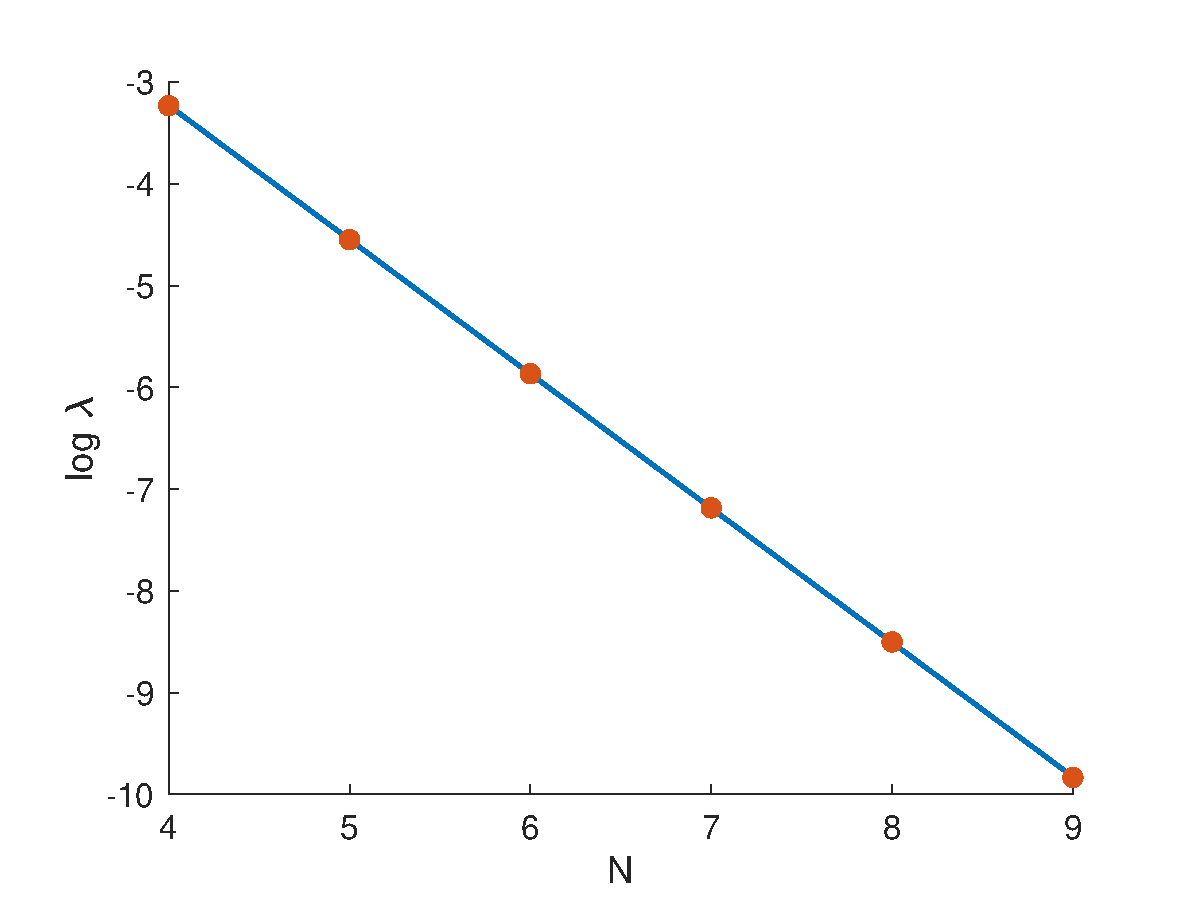
\includegraphics[width=10cm]{eigendecay.eps}
\label{fig:eigendecay}
\caption{Log of eigenvalue vs. $N$ for double pulses of dNLS. Parameters $\omega = 2$ and $\epsilon = 1.1$}
\end{figure}
The slope of the best-fit line is $-1.319$, which is a relative error of less than $0.05$ from $-\log r$.

\section{Proof of Existence Theorems}

\subsection{Discrete Exponential Dichotomy}

In this section, we state results about exponential dichotomies in the discrete setting. First, we define the discrete evolution operator for linear difference equations.

% lemma : discrete evolution operator
\begin{lemma}[Discrete Evolution Operator]\label{evolop}
Consider the difference equation together with its adjoint
\begin{align}
V(n+1) &= A(n) V(n) \label{diffeqevol} \\
Z(n+1) &= [A(n)^{-1}]^* Z(n) \label{adjeqevol}
\end{align}
where $n \in \Z$, $V(n) \in R^d$, and the $d \times d$ matrix $A(n)$ is invertible for all $n$. Define the discrete evolution operator by
\begin{equation}\label{evol}
\Phi(m, n) = 
\begin{cases}
I & m = n \\
A(m-1) \dots A(n+1) A(n) & m > n \\
A^{-1}(m) \dots A^{-1}(n-2) A^{-1}(n-1) & m < n
\end{cases}
\end{equation}
The evolution operators of \eqref{diffeqevol} and \eqref{adjeqevol} are related by
\begin{equation}\label{adjevol}
\Psi(m, n) = \Phi(n, m)^*
\end{equation}
Finally, if $V(n)$ is a solution to \eqref{diffeqevol} and $Z(n)$ is a solution to \eqref{adjeqevol}, then the inner product $\langle V(n), Z(n) \rangle$ is constant in $n$.

\begin{proof}
Since to evolve a difference equation we iterate a map (or its inverse) a finite number of times, the definition makes sense. We can easily check that this defines a flow. Let $\Psi(m, n)$ be the evolution operator for the adjoint equation \eqref{adjeqevol}. Then since $Z(n) = A(n)^* Z(n+1)$, for $m < n$ we have
\begin{align*}
\Psi(m, n) &= A(m)^* \dots A(n-2)^* A(n-1)^* \\
&= [A(n-1) A(n-2) \dots A(m)]^* \\
&= \Phi(n, m)^*
\end{align*}
We can similarly show that this holds for $m > n$, and it holds trivially for $m = n$.

For a solution $V(n)$ to \eqref{diffeqevol} and a solution $Z(n)$ to \eqref{adjeqevol},
\begin{align*}
\langle V(n+1), Z(n+1) \rangle &= 
\langle A(n) V(n), [A(n)^{-1}]^* Z(n) \rangle \\
&= \langle A(n)^{-1} A(n) V(n), Z(n) \rangle \\
&= \langle V(n), Z(n) \rangle
\end{align*}
Similarly, we can show that $\langle V(n+1), Z(n+1) \rangle = \langle V(n), Z(n) \rangle$.
\end{proof}
\end{lemma}

In the next lemma, we give a criterion for an exponential dichotomy in the discrete case.

% lemma : exp dichotomy in discrete case
\begin{lemma}[Exponential Dichotomy]\label{dichotomy}
Consider the difference equation
\begin{equation}\label{diffeqdichot}
V(n+1) = A(n) V(n)
\end{equation}
with evolution operator $\Phi(m, n)$ as defined in Lemma \ref{evolop}. Suppose that $A(n) \rightarrow A^\pm$ exponentially as $n \rightarrow \pm \infty$, i.e. there exist constants $r_\pm < 1$ such that
\begin{align*}
|A(n) - A^\pm| \leq C r_\pm^{|n|}
\end{align*}
where $A^\pm$ are constant coefficient matrices. If $A^\pm$ are hyperbolic, then \eqref{diffeqdichot} has exponential dichotomies on $Z^\pm$. In other words, there exist projections $P_\pm^s$ and $P_\pm^u$ defined on $\Z^\pm$ such that
\begin{equation}\label{projcommute}
P_\pm^{s/u}(m) \Phi(m, n) =  \Phi(m, n) P_\pm^{s/u}(n)
\end{equation}
Letting $\Phi_\pm^{s/u}(m, n) = \Phi(m, n) P_\pm^{s/u}(n)$ for $m, n \geq 0$ and $m, n \leq 0$ (respectively), we have the estimates
\begin{align*}
|\Phi_+^s(m, n)| \leq C (r_+^s)^{m - n} && 0 \leq n \leq m \\
|\Phi_+^u(m, n)| \leq C \left( \dfrac{1}{r_+^u} \right)^{n-m} && 0 \leq m \leq n \\
|\Phi_-^s(m, n)| \leq C (r_-^s)^{m - n} && n \leq m \leq 0 \\
|\Phi_-^u(m, n)| \leq C \left( \dfrac{1}{r_-^u} \right)^{n-m} && m \leq n \leq 0\\
\end{align*}
for constants $r_\pm^s < 1$, $r_\pm^u > 1$ which are chosen so that $|\lambda_\pm| \leq r_\pm^s < 1$ or $|\lambda_\pm| \geq r_\pm^u > 1$ for all eigenvalues $\lambda_\pm$ of $A^\pm$. 
 
Finally, let $E_\pm^{s/u}$ be the stable and unstable eigenspaces of $A^\pm$ and $Q_\pm^{s/u}$ the corresponding eigenprojections. Then we have
\begin{align*}
\dim \text{range }P_\pm^s(n) &= \dim E_\pm^s \\
\dim \text{range }P_\pm^u(n) &= \dim E_\pm^u
\end{align*}
and the decay rate
\begin{align}\label{projbound}
| P_\pm^{s/u}(n) - Q_\pm^{s/u} | \leq C r_\pm^{|n|}
\end{align}

\begin{proof}
We will consider the problem on $\Z^+$. The problem on $\Z^-$ is similar. Since $A^+$ is constant coefficient and hyperbolic, the difference equation $W(n+1) = A^+ W(n)$ has an exponential dichotomy on $\R^+$. Specifically, since $A^+$ is hyperbolic, we can find radii $r_+^s < 1$ and $r_+^u > 1$ such that for all eigenvalues $\lambda$ of $A^+$ either $|\lambda| \leq r_+^s$ or $|\lambda| \geq r_+^u$. Let $E_+^{s/u}$ be the stable and unstable eigenspaces of $A^+$, and let $P_+^{s/u}$ be the corresponding eigenprojections, which commute with $A^+$. Let $\Phi_+(m, n)$ be the evolution operator for $W(n+1) = A^+ W(n)$. Then we have bounds for the evolution operator
\begin{align*}
\Phi_+(m, n) P_+^s W &= (A^+)^{m-n} P_+^s W \leq C (r_+^s)^{m-n} W  && m > n \\
\Phi_+(m, n) P_+^u W &= [(A^+)^{-1}]^{n-m} P_+^u W \leq C \left( \dfrac{1}{r_+^s} \right)^{n-m} W && m < n
\end{align*}
where we used the fact that the stable eigenspace of $(A^+)^{-1}$ is equal to the unstable eigenspace of $A^-$ (and vice versa), and the eigenvalues of $(A^+)^{-1}$ and $A^-$ are reciprocals of each other.

Since $A(n) \rightarrow A^+$ as $n \rightarrow \infty$, by Proposition 2.5 in Beyn97, \eqref{diffeqdichot} has an exponential dichotomy on $\Z^+$, as defined in Beyn97, with the same constants $r_+^s$, $r_+^s$, and $C$. Furthermore, the range of $P_+^s(n)$ has the same dimension as $E_+^s$, and the range of $P_+^u(n)$ has the same dimension as $E_+^u$.

The estimate \eqref{projbound} should hold since we $A(n)$ is exponentially asymptotic to $A^+$. We are essentially replacing the ordinary decay in (17) and (18) of Beyn97 with exponential decay. There is probably another reference we can cite for this. By the same argument we have a corresponding exponential dichotomy on $\Z^-$.
\end{proof}
\end{lemma}

The last thing we will need is a version of the variation of constants formula for the discrete setting.

\begin{lemma}[Variation of Constants Formula]\label{VOC}
Consider the initial value for the difference equation
\begin{align*}
V(n+1) &= A(n) V(n) + G(V(n), n) \\
V(n_0) &= V_{n_0}
\end{align*}
The solution is given by
\begin{equation}\label{VOCformula}
V(n) = 
\begin{cases}
V_{n_0} & n = n_0 \\
\Phi(n, n_0) V_{n_0} + \sum_{j = n_0}^{n-1} \Phi(n, j+1) G(V(j), j)) & n > n_0 \\
\Phi(n, n_0) V_{n_0} - \sum_{j = n}^{n_0-1} \Phi(n, j+1) G(V(j), j)) & n < n_0 
\end{cases}
\end{equation}
\begin{proof}
For $n = n_0 + 1$,
\[
V(n_0 + 1) = A(n_0) V(n_0) + G(V(v_0), n_0) = \Phi(n_0+1, n_0) V_{n_0} + \Phi(n_0, n_0) G(V(v_0), n_0)
\]
Iterate this to get the result for $n > n_0$. The case for $n < n_0$ is similar.
\end{proof}
\end{lemma}

\subsection{Fixed Point Formulation}

First, we derive a formula for the family of evolution operators we will need in terms of the evolution operator for the variational equation.

\begin{lemma}\label{thetaevol}
Let $\Phi(m, n; \theta)$ be the evolution operator for 
\begin{equation}\label{Vtheta}
V(n+1; \theta) = DF(T(\theta)Q(n)) V(n; \theta) 
\end{equation}
Then $\Phi(m, n; \theta) = T(\theta)\Phi(m, n; 0)T(\theta)^{-1}$.
\begin{proof}
Differentiating the symmetry $F(T(\theta)U) = T(\theta)F(U)$ with respect to $U$, we have 
\[
DF(T(\theta)U)T(\theta) = T(\theta)DF(U)
\]
from which it follows that
\begin{equation}\label{DFtheta}
DF(T(\theta)Q(n)) = T(\theta)DF(Q(n))T(\theta)^{-1}
\end{equation}
From the definition of the evolution operator from Lemma \ref{evolop},
\[
\Phi(m, n; \theta) = T(\theta)\Phi(m, n; 0)T(-\theta)
\]
\end{proof}
\end{lemma}

Since $Q(n)$ decays exponentially to 0 at $\pm \infty$ and $T(\theta)$ is an isometry, the matrix $A(n; \theta) = DF(T(\theta) Q(n))$ in \eqref{Vtheta} is exponentially asymptotic to the constant coefficient matrix $A_\infty = DF(0)$, which is hyperbolic by Hypothesis \ref{initialhyp} and does not depend on $\theta$. Using Lemma \ref{dichotomy}, let $P_{s/u}^\pm(m; \theta)$ and $\Phi_{s/u}^\pm(m, n; \theta)$ be the projections and evolutions of the exponential dichotomy for the ODE \ref{Vtheta}. We note that the estimates from this lemma do not depend on $\theta$. Furthermore, if we take Hypothesis \ref{intersectionhyp}(ii), $T(\theta)S_1(n)$ is a solution to \eqref{Vtheta}.

We write equation \eqref{Wsystem1} in fixed-point form using the discrete variation of constants formula from Lemma \ref{VOCformula}.
\begin{equation}\label{FPeqs1}
\begin{aligned}
W_i^-(n) &= 
\Phi_s^-(n, -N_{i-1}^-; \theta_i) a_{i-1}^- + \Phi_u^-(n, 0; \theta_i) b_i^-  \\
&+ \sum_{j = -N_{i-1}^-}^{n-1} \Phi_s^-(n, j+1; \theta_i) G_i^-(W_i^-(j)) - \sum_{j = n}^{-1} \Phi_u^-(n, j+1; \theta_i) G_i^-(W_i^-(j)) \\
W_i^+(n) &= \Phi_u^+(n, N_i^+; \theta_i) a_i^+ + \Phi_s^+(n, 0; \theta_i) b_i^+ \\
&+ \sum_{j = 0}^{n-1} \Phi_s^+(n, j+1; \theta_i) G_i^+(W_i^+(j)) 
- \sum_{j = n}^{N_i^+-1} \Phi_u^+(n, j+1; \theta_i) G_i^+(W_i^+(j))
\end{aligned}
\end{equation}
where 
\begin{enumerate}
\item $a_i^- \in E^s$, $a_i^+ \in E^u$, and $a_0^- = a_m^+ = 0$
\item $b_i^+ \in T(\theta_i) Y^+$ and $b_i^- \in T(\theta_i) Y^-$
\item $W_i^-(n) \in l^\infty([-N_{i-1}^-, 0])$ and $W_i^+(n) \in l^\infty([0, N_i^+])$
\end{enumerate}

Since we are constructing a homoclinic orbit to the rest state at 0, we must take the initial conditions $a_0^- = 0$ and $a_m^+ = 0$. In these cases, the fixed point equations are given by
\begin{align*}
W_1^-(n) &= \Phi_u^-(n, 0; \theta_i) b_i^- 
+ \sum_{j = -\infty}^{n-1} \Phi_s^-(n, j+1; \theta_i) G_i^-(W_i^-(j)) - \sum_{j = n}^{-1} \Phi_u^-(n, j+1; \theta_i) G_i^-(W_i^-(j)) \\
W_m^+(n) &= \Phi_s^+(n, 0; \theta_i) b_i^+ 
+ \sum_{j = 0}^{n-1} \Phi_s^+(n, j+1; \theta_i) G_i^+(W_i^+(j)) 
- \sum_{j = n}^\infty \Phi_u^+(n, j+1; \theta_i) G_i^+(W_i^+(j))
\end{align*}
where the infinite sums converge due to the exponential dichotomy. 

We note that if Hypothesis \ref{intersectionhyp}(ii) holds, we do not need to include a component in $T(\theta_i) S_1$ in $b_i^\pm$, since that direction is taken care of by the symmetry parameter $\theta_i$.

\subsection{Inversion}

As in San98, we will solve equations \eqref{Wsystem1}, \eqref{Wsystem2}, and \eqref{Wsystem3} in stages. The first two steps are the same regardless of whether we take Hypothesis \ref{intersectionhyp}(i) or \ref{intersectionhyp}(ii). In the first lemma of this section, we solve for $W_i^\pm$. 

% solve for W
\begin{lemma}\label{inv1}
There exist unique bounded functions $W_i^\pm(n)$ such that equation \eqref{Wsystem1} is satisfied. These solutions depend smoothly on the initial conditions $a_i^\pm$ and $b_i\pm$, and we have the estimates.
\begin{equation}\label{Wipmest}
\begin{aligned}
||W_i^-|| &\leq C (|a_{i-1}^-| + |b_i^-|) \\
||W_i^+|| &\leq C (|a_i^+| + |b_i^+| )
\end{aligned}
\end{equation}
For the interior pieces, we have the piecewise estimates
\begin{equation}\label{Wipiecewise}
\begin{aligned}
|W_i^-(n)| &\leq C (r^{-(N_{i-1}^- + n)}|a_{i-1}^-| + r^n|b_i^-|) && n \in [-N_{i-1}^-, 0] \\
|W_i^+(n)| &\leq C (r^{-(N_i^+ - n)}|a_i^+| + r^{-n}|b_i^+| ) && n \in [0, N_i^+] 
\end{aligned}
\end{equation}

\begin{proof}
First, we show that the RHS of the fixed point equations \eqref{FPeqs1} defines a smooth map from $l^\infty$ (on the appropriate interval) to itself. We will verify the ``minus'' pieces; the ``plus'' pieces will be similar.

For the terms not involving sums, we have
\begin{align*}
|\Phi_s^-(n, &-N_{i-1}^-; \theta_i) a_{i-1}^-| + |\Phi_u^-(n, 0; \theta_i) b_i^-| \\
&\leq C ( r^{-(n + N_{i-1}^-)} |a_{i-1}^-| +  r^{-n}|b_i^-|) \\
&\leq C ( |a_{i-1}^-| + |b_i^-|) 
\end{align*}
which is independent of $n$. For the terms involving sums, we have
\begin{align*}
&\left| \sum_{j = -N_{i-1}^-}^{n-1} \Phi_s^-(n, j+1; \theta_i) G_i^-(W_i^-(j))\right| + \left|\sum_{j = n}^{-1} \Phi_u^-(n, j+1; \theta_i) G_i^-(W_i^-(j))\right| \\
&\leq C ||W_i^-||_{l^\infty([-N_{i-1}, 0])}^2 \left( \sum_{j = -N_{i-1}^-}^{n-1} r^{-(n - j - 1)} + \sum_{j = n}^{-1} r^{-(n - j - 1)} \right) \\
&= C ||W_i^-||_{l^\infty([-N_{i-1}, 0])}^2 \sum_{j = -N_{i-1}^-}^{-1} r^{-(n - j - 1)} \\
&= C ||W_i^-||_{l^\infty([-N_{i-1}, 0])}^2 r^{-n} \sum_{j = 0}^{N_{i-1} - 1} r^{-j} \\
&\leq C ||W_i^-||_{l^\infty([-N_{i-1}, 0])}^2 
\end{align*}
which is finite and also independent of $n$. Define the map $H_i^-: l^\infty([-N_{i-1}, 0]) \times E^s \times Y^- \rightarrow l^\infty([-N_{i-1}, 0])$ by
\begin{align*}
H_i^-(W_i^-(n), &a_{i-1}^-, b_i^-) = W_i^-(n) - \Phi_s^-(n, -N_{i-1}^-; \theta_i) a_{i-1}^- - \Phi_u^-(n, 0; \theta_i) b_i^-  \\
&- \sum_{j = -N_{i-1}^-}^{n-1} \Phi_s^-(n, j+1; \theta_i) G_i^-(W_i^-(j)) + \sum_{j = n}^{-1} \Phi_u^-(n, j+1; \theta_i) G_i^-(W_i^-(j)) 
\end{align*}
Since 0 is an equilibrium, $H(0, 0, 0) = 0$. We can check that the Fr\'echet derivative of $H_i^-$ with respect to $W_i^-$ at $(W_i^-(n), a_{i-1}^-, b_i^-) = (0, 0, 0)$ is a Banach space isomorphism on $l^\infty([-N_{i-1}, 0])$. Using the implicit function theorem, we can solve for $W_i^-(x)$ in terms of $(a_{i-1}^-, b_i^-)$. This dependence is smooth, since the map $H_i^-$ is smooth. The estimate \eqref{Wipmest} on $W_i^\pm$ comes from the terms in the fixed point equations which do not involve sums, since the terms involving sums are quadratic in $W_i^\pm$. For the interior pieces, we can similarly obtain the piecewise estimates
\begin{align*}
|W_i^-(n)| &\leq C (r^{-(N_{i-1}^- + n)}|a_{i-1}^-| + r^n|b_i^-|) && n \in [-N_{i-1}^-, 0] \\
|W_i^+(n)| &\leq C (r^{-(N_i^+ - n)}|a_i^+| + r^{-n}|b_i^+| ) && n \in [0, N_i^+] 
\end{align*}
\end{proof}
\end{lemma}

Next, we use the center matching conditions at $N_i^\pm$ to solve for the initial conditions $a_i^\pm$.

% match in middles
\begin{lemma}\label{inv2}
For $i = 1, \dots m-1$ there is a unique pair of initial conditions $(a_i^+, a_i^-) \in E^u \times E^s$ such that the matching conditions \eqref{Wsystem2} are satisfied. $(a_i^+, a_i^-)$ depends smoothly on $(b_i^+, b_{i+1}^-)$, and we have the following expressions for $a_i^-$ and $a_i^+$. 
\begin{equation}\label{aipmest}
\begin{aligned}
a_i^+ &= P_0^u d_i + \tilde{a}_i^+ \\
a_i^- &= -P_0^s d_i + \tilde{a}_i^-
\end{aligned}
\end{equation}
where 
\begin{equation}\label{tildeaest}
\tilde{a}_i^\pm = \mathcal{O}(r^{-N}(|b_i^+|+|b_{i+1}^-|) + |b_i^+|^2+|b_{i+1}^-|^2) 
\end{equation}
In terms of $Q(\pm N_i^\pm)$, we can write \eqref{aipmest} as 
\begin{equation}\label{aipmexp}
\begin{aligned}
a_i^- &= T(\theta_i) Q(N_i^+) + \tilde{a}_i^- + \mathcal{O}(r^{-2N}) \\
a_i^+ &= T(\theta_{i+1}) Q(-N_i^-) + \tilde{a}_i^+ + \mathcal{O}(r^{-2N}) \\
\end{aligned}
\end{equation}

\begin{proof}
Evaluating the fixed point equations \eqref{FPeqs1} at $\pm N_i^\pm$ and subtracting, we need to solve
\begin{align*}
d_i &= W_i^+(N_i^+) - W_{i+1}^-(-N_i^-) \\
&= P_u^+(N_i^+; \theta_i) a_i^+ + \Phi_s^+(N_i^+, 0; \theta_i) b_i^+ + \sum_{j = 0}^{N_i^+-1} \Phi_s^+(N_i^+, j+1; \theta_i) G_i^+(W_i^+(j)) \\
&-P_s^-(-N_i^-; \theta_{i+1}) a_i^- - \Phi_u^-(-N_i^-, 0; \theta_{i+1}) b_{i+1}^-
- \sum_{j = -N_i^-}^{-1} \Phi_u^-(-N_i^-, j+1; \theta_{i+1}) G_i^-(W_i^-(j))
\end{align*}
Define $H_i: E^s \times E^u \times Y^+ \times Y^- \times \rightarrow \R^d$ by
\begin{align*}
H_i(a_i^+, &a_i^-, b_i^+, b_{i+1}^-) \\
&= a_i^+ - a_i^- - d_i + (P_u^+(N_i^+; \theta_i) - P_0^u) a_i^+ - (P_s^-(-N_i^-; \theta_{i+1}) - P_0^s) a_i^- \\
&+ \Phi_s^+(N_i^+, 0; \theta_i) b_i^+ - \Phi_u^-(-N_i^-, 0; \theta_{i+1}) b_{i+1}^- \\
&+ \sum_{j = 0}^{N_i^+-1} \Phi_s^+(N_i^+, j+1; \theta_i) G_i^+(W_i^+(j; a_i^+, b_i^+)) \\
&+ \sum_{j = -N_i^-}^{-1} \Phi_u^-(-N_i^-, j+1; \theta_{i+1}) G_i^-(W_{i+1}^-(j; a_i^-, b_{i+1}^-))
\end{align*}
where we substituted $W_{i+1}^-(n; a_i^-, b_{i+1}^-)$ and $W_i^+(n; a_i^+, b_i^+)$ from the previous lemma. Since $(a_i^+, a_i^-) \in E^s \oplus E^u = \R^d$, we can use the IFT. First, we note that $H_i(0,0,0,0) = 0$. Next, we differentiate $H_i$ with respect to $a_i^\pm$. When we do this, the derivatives of the terms involving sums will be 0 since $G_i^\pm$ is quadratic in $W_i^\pm$, thus quadratic order in $a_i^\pm$ by Lemma \ref{inv1}. Thus the partial derivative with respect to $a_i^\pm$ at $(a_i^+, a_i^-, b_i^+, b_{i+1}^-) = (0, 0, 0, 0)$ is 
\begin{align*}
\frac{\partial}{\partial a_i^-} H_i(0, 0, 0, 0) &= \pm 1 + \mathcal{O}(r^{-N_i^-}) \\
\frac{\partial}{\partial a_i^+} H_i(0, 0, 0, 0) &= \pm 1 + \mathcal{O}(r^{-N_i^+})
\end{align*}
For sufficiently large $N$, $D_{a_i^\pm} H(0, 0, 0, 0, 0)$ is invertible in a neighborhood of $(0, 0, 0, 0, 0)$, thus we can use the IFT to solve for $a_i^\pm$ in terms of $(b_i^+$, $b_{i+1}^-)$ for $(b_i^+, b_{i+1}^-)$ sufficiently small.

To get the estimates on and expressions for $a_i^\pm$, we note that we solved the equation $H_i(a_i^+, a_i^-, b_i^+, b_{i+1}^-) = 0$, which is of the form
\begin{align*}
0 &= a_i^+ - a_i^- - d_i + \mathcal{O}(r^{-N}(|a_i^+|+|a_i^-|+|b_i^+|+|b_{i+1}^-|)\\
&+ \mathcal{O}((|a_i^+|^2+|a_i^-|^2+|b_i^+|^2+|b_{i+1}^-|^2)
\end{align*}
Taking projections on $E^s$ and $E^u$, we have
\begin{align*}
a_i^+ &= P_0^u d_i + \mathcal{O}(r^{-N}(|b_i^+|+|b_{i+1}^-|) + |b_i^+|^2+|b_{i+1}^-|^2) \\
a_i^- &= -P_0^s d_i + \mathcal{O}(r^{-N}(|b_i^+|+|b_{i+1}^-|) + |b_i^+|^2+|b_{i+1}^-|^2)
\end{align*}
We can write this as 
\begin{align*}
a_i^+ &= P_0^u d_i + \tilde{a}_i^+ \\
a_i^- &= -P_0^s d_i + \tilde{a}_i^-
\end{align*}
where
\[
\tilde{a}_i^\pm = \mathcal{O}(r^{-N}(|b_i^+|+|b_{i+1}^-|) + |b_i^+|^2+|b_{i+1}^-|^2) 
\]

To obtain expressions in terms of $Q(\pm N_i^\pm)$, we note that
\begin{align*}
P_0^s T(\theta_i) Q(N_i^+) &= (P_0^s - P_s^+(N_i^+; \theta_i)) T(\theta_i) Q(N_i^+) + P_s^+(N_i^+; \theta_i) T(\theta_i) Q(N_i^+) \\
&= P_s^+(N_i^+; \theta_i) T(\theta_i) Q(N_i^+) + \mathcal{O}(r^{-2N}) \\
&= T(\theta_i) Q(N_i^+) + \mathcal{O}(r^{-2N}) 
\end{align*}
and 
\begin{align*}
P_0^s T(\theta_{i+1}) Q(-N_i^-) 
&= P_0^s \Big( ( P_u^-(-N_i^-; \theta_{i+1}) - P_0^u) T(\theta_{i+1}) Q(-N_i^-) + P_0^u T(\theta_{i+1}) Q(-N_i^-) \Big) \\
&= P_0^s ( P_u^-(-N_i^-; \theta_{i+1}) - P_0^u) T(\theta_{i+1}) Q(-N_i^-) + P_0^s P_0^u T(\theta_{i+1}) Q(-N_i^-) \\
&= \mathcal{O}(r^{-2N})
\end{align*}
Using these, we obtain
\begin{align*}
a_i^- &= T(\theta_i) Q(N_i^+) + \tilde{a}_i^- + \mathcal{O}(r^{-2N})
\end{align*}
Similarly, we have
\begin{align*}
a_i^+ &= T(\theta_{i+1}) Q(-N_i^-) + \tilde{a}_i^+ + \mathcal{O}(r^{-2N}) \\
\end{align*}
\end{proof}
\end{lemma}

It only remains to solve \eqref{Wsystem3}. Here, the two cases from Hypothesis \ref{intersectionhyp} are very different.

First, we consider the transverse intersection case, i.e. we assume Hypothesis \ref{intersectionhyp}(i). In this case, existence of the multi-pulse solution is a straightforward application of the implicit function theorem.

% center match, transverse intersection
\begin{lemma}\label{inv3t}
Assume Hypothesis \ref{intersectionhyp}(i). Then for $i = 1, \dots m$ there is a unique pair of initial conditions $(b_i^-, b_i^+) \in T(\theta_i) Y^- \times T(\theta_i) Y^+$ such that the matching conditions \eqref{Wsystem3} are satisfied. We have the uniform bound
\begin{equation}\label{bboundt}
b = \mathcal{O}(r^{-2N})
\end{equation}

\begin{proof}
Evaluating the fixed point equations \eqref{FPeqs1} at 0 and subtracting, we have
\begin{align*}
W_i^+(0) &- W_i^-(0) = b_i^+ - b_i^- 
+ \Phi_u^+(0, N_i^+; \theta_i) a_i^+ - \Phi_s^-(0, -N_{i-1}^-; \theta_i) a_{i-1}^- \\
&- \sum_{j = 0}^{N_i^+-1} \Phi_u^+(0, j+1; \theta_i) G_i^+(W_i^+(j)) 
- \sum_{j = -N_{i-1}^-}^{-1} \Phi_s^-(0, j+1; \theta_i) G_i^-(W_i^-(j)) \\
\end{align*}
Next, substitute $W_i^\pm$ from Lemma \ref{inv1} and $a_i^\pm$ from Lemma \ref{inv2}. Define the spaces
\begin{align}\label{spaceYt}
Y &= \bigoplus_{i=1}^m (T(\theta) Y^+ \oplus T(\theta) 2Y^-) = \bigoplus_{i=1}^m \R^d \\
Z &= \bigoplus_{i=1}^{m-1} \R^d
\end{align}
Let $b = (b_1^+, b_1^-, \dots, b_m^+, b_m^-) \in Y$ and $d = (d_1, \dots, d_{m-1}) \in Z$. Define the function $H: Y \times Z \rightarrow Y$ component-wise by
\begin{align*}
H_i(b, d) &= 
 b_i^+ - b_i^- + \Phi_u^+(0, N_i^+; \theta_i) P_0^u d_i + \Phi_s^-(0, -N_{i-1}^-; \theta_i) P_0^s d_{i-1} \\
&+ \Phi_u^+(0, N_i^+; \theta_i) \tilde{a}_i^+(b_i^+, b_{i+1}^-) 
- \Phi_s^-(0, -N_{i-1}^-; \theta_i) \tilde{a}_{i-1}^-(b_{i-1}^+, b_i^-) \\
&- \sum_{j = 0}^{N_i^+-1} \Phi_u^+(0, j+1; \theta_i) G_i^+(W_i^+(j; b_i^+, b_{i+1}^-)) \\
&- \sum_{j = -N_{i-1}^-}^{-1} \Phi_s^-(0, j+1; \theta_i) G_i^-(W_i^-(j; b_{i-1}^+, b_i^-))
\end{align*}

where $d_0 = d_m = 0$, and we have indicated the dependencies on the $b_i^\pm$. From \eqref{spaceYt}, we are set up to use the implicit function theorem. Using the estimates from Lemmas \ref{inv1} and \ref{inv2}, $H(0, 0) = 0$. For the partial derivatives with respect to $b_i^\pm$, we have
\begin{align*}
\frac{\partial}{\partial b_i^+}H_i(0) &= 1 + \mathcal{O}(r^{-N})  \\
\frac{\partial}{\partial b_i^-}H_i(0) &= -1 + \mathcal{O}(r^{-N}) \\
\frac{\partial}{\partial b_{i-1}^+}H_i(0),
\frac{\partial}{\partial b_{i+1}^-}H_i(0) &= \mathcal{O}(r^{-N}) \\
\end{align*}
and 
\[
\frac{\partial}{\partial b_j^\pm}H_i(0) = 0
\]
for all other indices. Thus, for sufficiently large $N$, the matrix $D_b H(0,0)$ is invertible. Using the implicit function theorem, we can solve for $b$ in terms of $d$ for near $(b,d) = (0, 0)$, i.e. there is a function $b: Z \rightarrow Y$ with $b(0) = 0$ such that $H(b(d),d) = 0$ for $d$ sufficiently small. Since $d = \mathcal{O}(r^{-N}$, we can do this as long as $N$ is sufficiently large.

To find a bound for $b$, recall that we use the IFT to solve $H(b(d),d) = 0$, which, component-wise, has the form
\begin{align*}
0 &= b_i^+ - b_i^- + \mathcal{O}(r^{-N_i^+} d_i + r^{-N_{i-1}^-} d_{i-1}) \\
&+ \mathcal{O}( r^{-N}(|b_i^+| + |b_i^-| + |b_{i+1}^-| + |b_{i-1}^+|)
+ (|b_i^+|^2 + |b_i^-|^2 + |b_{i+1}^-|^2 + |b_{i-1}^+|^2)
\end{align*}
Since $b$ is small and $d = \mathcal{O}(r^{-N})$, we have the bound
\[
b = \mathcal{O}(r^{-2N})
\]
\end{proof}
\end{lemma}

For the non-transverse intersection case, we will not have such a straightforward result, i.e. we will not in general be able to uniquely solve equation \eqref{Wsystem3}. Instead, we will obtain a set of jump conditions in the direction of $T(\theta) Z_1(0)$ which will depend on the symmetry parameters $\theta_i$. Recall that we have the decomposition
\[
\R^d = \R S_1(0) \oplus Y^+ \oplus Y^- \oplus \R Z_1(0)
\]
Thus, projecting in these directions, we can write \eqref{Wsystem3} as the system of equations

\begin{align}
P_{T(\theta)S_1}\left( W_i^+(0) - W_i^-(0) \right) &= 0 \label{jumpS1} \\
P_{T(\theta)Y^+ \oplus T(\theta)Y^-}\left( W_i^+(0) - W_i^-(0) \right) &= 0 \label{jumpnonZ} \\
P_{\R T(\theta)Z_1(0)} \left( W_i^+(0) - W_i^-(0) \right) &= 0 \label{jumpZ}
\end{align}

Since by \eqref{W0loc} we were able to choose $W_i^\pm$ such that $W_i^\pm(0) \in Y^+ \oplus Y^- \oplus \R Z_1(0)$, equation \ref{jumpS1} is automatically satisfied. Since $b_i^+ \in T(\theta) Y^+$ and $b_i^- \in T(\theta) Y^-$, we will be able to satisfy \eqref{jumpnonZ} by solving for the $b_i^\pm$, which we do in the following lemma.

% solve for $b_i^\pm$, nontransverse int
\begin{lemma}\label{inv3nt}
Assume Hypothesis \ref{intersectionhyp}(ii). Then for $i = 1, \dots m$ there is a unique pair of initial conditions $(b_i^-, b_i^+) \in T(\theta_i) Y^- \times T(\theta_i) Y^+$ such that the jump conditions \eqref{jumpnonZ} are satisfied. We have the uniform bound
\begin{equation}\label{bboundt}
b = \mathcal{O}(r^{-2N})
\end{equation}

\begin{proof}
Evaluating the fixed point equations \eqref{FPeqs1} at 0 and subtracting, we have
\begin{align*}
W_i^+(0) &- W_i^-(0) = b_i^+ - b_i^- 
+ \Phi_u^+(0, N_i^+; \theta_i) a_i^+ - \Phi_s^-(0, -N_{i-1}^-; \theta_i) a_{i-1}^- \\
&- \sum_{j = 0}^{N_i^+-1} \Phi_u^+(0, j+1; \theta_i) G_i^+(W_i^+(j)) 
- \sum_{j = -N_{i-1}^-}^{-1} \Phi_s^-(0, j+1; \theta_i) G_i^-(W_i^-(j)) \\
\end{align*}
Substitute $W_i^\pm$ from Lemma \ref{inv1} and $a_i^\pm$ from Lemma \ref{inv2}, and project onto $T(\theta)Y^+ \oplus T(\theta)Y^-$. The remainder of the proof follows as in the proof of Lemma \ref{inv3t}.
\end{proof}
\end{lemma}

Finally, we will look at equation \ref{jumpZ}. As mentioned above, we will in general not be able to solve this equation uniquely. Instead, we will have $m$ jump conditions in the direction of $Z_1$ which will depend on the symmetry parameters $\theta_i$. We derive these jump conditions in the next lemma.

\begin{lemma}\label{jumpZlemma}
Assume Hypothesis \ref{intersectionhyp}(ii). Then the jump conditions in the direction of $Z_1$ are given by
\begin{equation}\label{jumpZ}
\begin{aligned}
\xi_1 &= \langle T(\theta_1) Z_1(N_1^+), T(\theta_2) Q(-N_1^-) \rangle + R_1  \\
\xi_i &= \langle T(\theta_i) Z_1(N_i^+), T(\theta_{i+1}) Q(-N_i^-) \rangle
- \langle T(\theta_i) Z_1(-N_{i-1}^-), T(\theta_{i-1}) Q(N_{i-1}^+) + R_i &&
i = 2, \dots, m-1 \\
\xi_m &= -\langle T(\theta_m) Z_1(-N_{m-1}^-), T(\theta_{m-1}) Q(N_{m-1}^+) + R_m
\end{aligned}
\end{equation}
for $i = 1, \dots, m$, where 
\[
|R_i| \leq C r^{-3N}
\]
\begin{proof}
Evaluating the fixed point equations \eqref{FPeqs1} at 0 and subtracting, we have
\begin{align*}
W_i^+(0) &- W_i^-(0) = b_i^+ - b_i^- 
+ \Phi_u^+(0, N_i^+; \theta_i) a_i^+ - \Phi_s^-(0, -N_{i-1}^-; \theta_i) a_{i-1}^- \\
&- \sum_{j = 0}^{N_i^+-1} \Phi_u^+(0, j+1; \theta_i) G_i^+(W_i^+(j)) 
- \sum_{j = -N_{i-1}^-}^{-1} \Phi_s^-(0, j+1; \theta_i) G_i^-(W_i^-(j)) \\
\end{align*}
Substitute \eqref{aipmest} from Lemma \ref{inv1} to get
\begin{align*}
W_i^+(0) &- W_i^-(0) = \Phi_u^+(0, N_i^+; \theta_i) P_0^u d_i + \Phi_s^-(0, -N_{i-1}^-; \theta_i) P_0^s d_{i-1} \\
&+ b_i^+ - b_i^- 
+ \Phi_u^+(0, N_i^+; \theta_i) \tilde{a}_i^+ - \Phi_s^-(0, -N_{i-1}^-; \theta_i) \tilde{a}_{i-1}^- \\
&- \sum_{j = 0}^{N_i^+-1} \Phi_u^+(0, j+1; \theta_i) G_i^+(W_i^+(j)) 
- \sum_{j = -N_{i-1}^-}^{-1} \Phi_s^-(0, j+1; \theta_i) G_i^-(W_i^-(j)) \\
\end{align*}
Now, project on $\R T(\theta_i) Z_1(0)$ by taking the inner product with $T(\theta_i) Z_1$. Since $b_i^\pm \in T(\theta_i) Y_i^\pm$, these terms are eliminated with the projection. For the leading order terms, we have
\begin{align*}
\langle T(\theta_i) Z_1(0), &\Phi_u^+(0, N_i^+; \theta_i) P_0^u d_i \rangle
= \langle \Phi_u^+(N_i^+, 0; \theta_i)^* T(\theta_i) Z_1(0), P_0^u d_i \rangle \\
&= \langle T(\theta_i) Z_1(N_i^+), P_0^u d_i \rangle \\
&= \langle T(\theta_i) Z_1(N_i^+), P_0^u T(\theta_{i+1}) Q(-N_i^-) - P_0^u T(\theta_i) Q(N_i^+) \rangle \\
&= \langle T(\theta_i) Z_1(N_i^+), P_-^u(-N_i^-; \theta_{i+1}) T(\theta_{i+1}) Q(-N_i^-) - P_0^u P_+^s(N_i^+; \theta_i)  T(\theta_i) Q(N_i^+) \rangle + \mathcal{O}(r^{-3N}) \\
&= \langle T(\theta_i) Z_1(N_i^+), T(\theta_{i+1}) Q(-N_i^-) - P_0^u P_0^s T(\theta_i) Q(N_i^+) \rangle + \mathcal{O}(r^{-3N}) \\
&= \langle T(\theta_i) Z_1(N_i^+), T(\theta_{i+1}) Q(-N_i^-) \rangle + \mathcal{O}(r^{-3N}) 
\end{align*}
Similarly,
\begin{align*}
\langle T(\theta_i) Z_1(0), &\Phi_s^-(0, -N_{i-1}^-; \theta_i) P_0^s d_{i-1} \rangle
= -\langle T(\theta_i) Z_1(-N_{i-1}^-), T(\theta_{i-1}) Q(N_{i-1}^+) \rangle + \mathcal{O}(r^{-3N}) 
\end{align*}

For the higher order terms, substitute $W_i^\pm$ from Lemma \ref{inv1}, $\tilde{a}_i^\pm$ from Lemma \ref{inv2}, and $b_i^\pm$ from Lemma \ref{inv3nt}. This gives us the following bounds.
\begin{enumerate}
	\item For the terms involving $\tilde{a}$, 
	\begin{align*}
	|\Phi_u^+(0, N_i^+; \theta_i) \tilde{a}_i^+| 
	&\leq C r^{-N} (r^{-N}(|b_i^+|+|b_{i+1}^-|) + |b_i^+|^2+|b_{i+1}^-|^2) \\
	&\leq C r^{-N} (r^{-N}r^{-2N} + r^{-4N}) \\
	&\leq C r^{-4N}
	\end{align*}
	The other term is similar.
	\item For the terms involving sums, since $G_i^\pm(U)$ is quadratic in $U$,
	\begin{align*}
	\left| \sum_{j = 0}^{N_i^+-1} \Phi_u^+(0, j+1; \theta_i) G_i^+(W_i^+(j)) \right|
	\leq C \sum_{j = 0}^{N_i^+-1} r^{-(j+1)}|W_i^+(j)|^2
	\end{align*}
	For the interior pieces, we use the piecewise estimates \eqref{Wipiecewise} from Lemma \ref{inv1} to get
	\begin{align*}
	\left| \sum_{j = 0}^{N_i^+-1} \Phi_u^+(0, j+1; \theta_i) G_i^+(W_i^+(j)) \right|
	&\leq C \sum_{j = 0}^{N_i^+-1} r^{-(j+1)}(r^{-(N_i^+ - j)}|a_i^+| + r^{-j}|b_i^+| )^2 \\
	&\leq C \sum_{j = 0}^{N_i^+-1} r^{-(j+1)}(r^{-2(N_i^+ - j)}|a_i^+|^2 + r^{-j}|b_i^+|^2) \\
	&\leq C \left( \sum_{j = 0}^{N_i^+-1} r^{-(j+1)}r^{-2(N_i^+ - j)}|a_i^+|^2 + \sum_{j = 0}^{N_i^+-1} r^{-(j+1)} r^{-2j}|b_i^+|^2 \right) \\
	&\leq C \left( \sum_{j = 0}^{N_i^+-1} r^{-1}r^{-(N_i^+ - j)}r^{-N_i^+}r^{-2N} + \sum_{j = 0}^{N_i^+-1} r^{-(j+1)} r^{-2j}r^{-4N} \right) \\
	&\leq C r^{-3N}
	\end{align*}
	The ``negative'' piece is similar. For the end pieces, we have for $W_m^+$
	\begin{align*}
	\left| \sum_{j = 0}^{N_m^+-1} \Phi_u^+(0, j+1; \theta_m) G_m^+(W_m^+(j)) \right|
	&\leq C \sum_{j = 0}^\infty r^{-(j+1)}|b_m^+|^2 \\
	&\leq C \sum_{j = 0}^\infty r^{-(j+1)}r^{-4N} \\
	&\leq C r^{-4N}
	\end{align*}
	The other end piece involving $W_1^-$ is similar.
\end{enumerate}
Combining these, we obtain the $m$ jump conditions
\[
\xi_i = \langle T(\theta_i) Z_1(N_i^+), T(\theta_{i+1}) Q(-N_i^-) \rangle
- \langle T(\theta_i) Z_1(-N_{i-1}^-), T(\theta_{i-1}) Q(N_{i-1}^+) + R_i
\]
where 
\[
|R_i| \leq C r^{-3N}
\]
Since $N_0^- = N_m^+ = \infty$, one of the two inner product terms vanishes in $\xi_1$ and $\xi_m$, leaving us with
\begin{align*}
\xi_1 &= \langle T(\theta_1) Z_1(N_1^+), T(\theta_2) Q(-N_1^-) \rangle + R_1  \\
\xi_i &= \langle T(\theta_i) Z_1(N_i^+), T(\theta_{i+1}) Q(-N_i^-) \rangle
- \langle T(\theta_i) Z_1(-N_{i-1}^-), T(\theta_{i-1}) Q(N_{i-1}^+) + R_i &&
i = 2, \dots, m-1 \\
\xi_m &= -\langle T(\theta_m) Z_1(-N_{m-1}^-), T(\theta_{m-1}) Q(N_{m-1}^+) + R_m
\end{align*}

\end{proof}
\end{lemma}

\subsection{Proofs of Theorems \ref{transversemulti} and \ref{ntmulti}}
The existence statement from Theorem \ref{transversemulti} follows from Lemma \ref{inv3t}, and the existence statement from Theorem \ref{ntmulti} follows from Lemma \ref{jumpZlemma}. The uniform bound $||W_i^\pm|| \leq C r^{-N}$follows from Lemma \ref{inv1} together with the estimates on $a_i^\pm$ and $b_i^\pm$. For the remaining estimates, recall that we have solved equation \eqref{Wsystem2}. Substituting \eqref{defdi} into \eqref{Wsystem2}, we have solved the equation
\begin{equation}\label{Wsubdi}
W_i^+(N_i^+) - W_{i+1}^-(-N_i^-) = T(\theta_{i+1}) Q(-N_i^-) - T(\theta_i) Q(N_i^+)
\end{equation}
Apply the projection $P^u_-(-N_i^-; \theta_{i+1})$ to both sides of \eqref{Wsubdi}, noting that it acts as the identity on $T(\theta_{i+1}) Q(-N_i^-)$. We look at the three remaining terms in \eqref{Wsubdi} one at a time. For $T(\theta_i) Q(N_i^+)$, we use Lemma \ref{dichotomy} to get
\begin{align*}
P^u_-(-N_i^-; \theta_{i+1})T(\theta_i) Q(N_i^+)
&= P^u_-(-N_i^-; \theta_{i+1}) P^s_+(N_i^+ \theta_i) T(\theta_i) Q(N_i^+) \\
&= P^u_0 P^s_+(N_i^+ \theta_i) T(\theta_i) Q(N_i^+) + \mathcal{O}(r^{-2N}) \\
&= P^u_0 P^s_0 T(\theta_i) Q(N_i^+) + \mathcal{O}(r^{-2N}) \\
&= \mathcal{O}(r^{-2N})
\end{align*}
For $W_i^+(N_i^+)$, we use the fixed point equations \eqref{FPeqs1} and the uniform bound on $W_i^\pm$ to get
\begin{align*}
(I - &P^u_-(-N_i^-; \theta_{i+1})) W_i^+(N_i^+) = P^s_-(-N_i^-; \theta_{i+1}) W_i^+(N_i^+) \\
&= P^s_0 W_i^+(N_i^+)W_i^+(N_i^+) + \mathcal{O}(r^{-2N}) \\
&= P^s_+(N_i^+; \theta_i)W_i^+(N_i^+) + \mathcal{O}(r^{-2N}) \\
&= P^s_+(N_i^+; \theta_i) P^u_+(N_i^+; \theta_i) a_i^+ + P^s_+(N_i^+; \theta_i) \left( \Phi_s^+(N_i^+, 0; \theta_i) b_i^+ + \sum_{j = 0}^{N_i^+-1} \Phi_s^+(n, j+1; \theta_i) G_i^+(W_i^+(j)) \right) \\
&= \mathcal{O}(r^{-2N})
\end{align*}
Thus we conclude 
\[
P^u_-(-N_i^-; \theta_{i+1}) W_i^+(N_i^+) = W_i^+(N_i^+) + \mathcal{O}(e^{-2N})
\]
For $W_{i+1}^-(-N_i^-)$, we use the fixed point equation \eqref{FPeqs1} and, following a similar procedure, conclude that
\[
P^u_-(-N_i^-; \theta_{i+1}) W_{i+1}^-(-N_i^-) = \mathcal{O}(e^{-2N})
\]
Combining all of these, we attain the bound
\[
W_i^+(N_i^+) = T(\theta_{i+1}) Q(-N_i^-) + \mathcal{O}(r^{-2N})
\]
Following the same method, but applying the projection $P^s_+(N_i^+; \theta_i)$ to both sides of \eqref{Wsubdi}, we also have the bound
\[
W_{i+1}^-(-N_i^-) = T(\theta_i) Q(N_i^+) + \mathcal{O}(r^{-2N})
\]

\section{Proof of Stability Theorem}

\subsection{Setup}

To prove the stability theorem, we will also use Lin's method. As in San98, we will write the eigenfunction as a piecewise perturbation of the symmetry eigenfunction $S_1(n)$. 

Assume Hypothesis \ref{initialhyp} and Hypothesis \ref{intersectionhyp}(ii). Using Theorem \ref{ntmulti}, let $Q_m(n)$ be an $m-$pulse solution to \eqref{diffeq} which resembles $m$ copies of the primary pulse solution $Q_1(n)$. We write $Q_m(n)$ piecewise as in \eqref{qmpiecewise}, and we have the following bounds from Theorem \ref{ntmulti}.
\begin{enumerate}[(i)]
\item $Q_1(n) = \mathcal{O}(r^n)$
\item $||\tilde{Q}|| \leq C r^N$
\item $|\tilde{Q}_{i+1}^-(-N_i^-) - T(\theta_i) Q_1(N_i^+)|| \leq C r^{2N}$ 
\item $|\tilde{Q}_i^+(N_i^+) - T(\theta_{i+1}) Q_1(-N_i^-)|| \leq C r^{2N}$
\end{enumerate}

Recall that the eigenvalue problem is given by 
\begin{align*}
V(n+1) = DF(Q_m(n)) V(n) + \lambda B V(n)
\end{align*}
Let $S_m(n) = S Q_m(n)$, where $S$ is the infinitesimal generator of the symmetry $T(\theta)$. Then $S_m(n)$ solves the equation
\begin{equation}\label{Smsolves}
S_m(n+1) = A(Q_m(n))S_m(n)
\end{equation}
Using the piecewise form of $Q_m(n)$ from \eqref{qmpiecewise}, we can write $S_m(n)$ piecewise as 
\begin{equation}\label{Smdef}
S_m(n) = S T(\theta_i) Q(n) + S \tilde{Q}_i^\pm(n)
= T(\theta_i) S_1(n) + \tilde{S}_i^\pm(n)
\end{equation}
where we use the fact that $S$ commutes with $T(\theta)$. Since $S$ is a bounded matrix, bounds from Theorem \ref{ntmulti} apply to $S_m(n)$ as well.

As in San98, we will take a piecewise ansatz for the eigenfunction $V(n)$. The form of the ansatz will depend on whether we take Hypothesis \ref{melnikovhyp}(i) or \ref{melnikovhyp}(ii). For Hypothesis \ref{melnikovhyp}(i), we use the piecewise ansatz
\begin{align*}
V_i^\pm(n) &= d_i S_m(n) + W_i^\pm(n) = d_i ( T(\theta_i) S_1(n) + \tilde{S}_i^\pm(n) ) + W_i^\pm(n)
&& i = 1, \dots, n-1
\end{align*}
where $d_i \in \C$. Substituting this into \eqref{latticeEVP} and simplifying, the eigenvalue problem becomes
\begin{equation}\label{EVPhypi}
W_i^\pm(n) = DF(Q_m(n)) W_i^\pm(n) + \lambda B W_i^\pm(n) + \lambda d_i B T(\theta_i) S_1(n) + \lambda d_i B \tilde{S}_i^\pm(n)
\end{equation}

If instead Hypothesis \ref{melnikovhyp}(ii) holds, recall that there exists a localized function $T_1(n)$ such that 
\begin{equation}\label{T1vareq}
T_1(n+1) = DF(Q(n)) T_1(n) + B S_1(n)
\end{equation}
Using the symmetry relation $F(T(\theta)U) = T(\theta)F(U)$ and the commuting relation $B T(\theta) = T(\theta)B$ from Hypothesis \ref{melnikovhyp}(ii), this we also have
\begin{equation}\label{TthetaT1vareq}
T(\theta)T_1(n+1) = DF(T(\theta)Q(n)) T(\theta)T_1(n) + B T(\theta) S_1(n)
\end{equation}
Similarly, by the Fredholm alternative, there exists a function $T_m(n)$ such that 
\begin{equation}\label{Tmsolves}
T_m(n+1) = DF(Q_m(n)) T_m(n) + B S_m(n)
\end{equation}
In this case, we use the piecewise ansatz
\begin{equation}\label{Viansatz2}
V_i^\pm(n) = 
d_i [ S_m(n) + \lambda T_m(n) ] + W_i^\pm(n)
\end{equation}
Substituting this into \eqref{latticeEVP}, we get
\begin{align*}
d_i &S_m(n+1) + d_i \lambda T_m(n+1) + W_i^\pm(n+1) \\
&= d_i DF(Q_m(n)) S_m(n) + d_i \lambda DF(Q_m(n)) T_m(n) + DF(Q_m(n)) W_i^\pm(n) \\
&+ d_i \lambda B S_m + d_i \lambda^2 B T_m(n) + \lambda B W_i^\pm(n)
\end{align*}
Using equations \eqref{Smsolves} and \eqref{Tmsolves}, this simplifies to
\begin{align*}
W_i^\pm(n+1)
&= DF(Q_m(n)) W_i^\pm(n) + \lambda B W_i^\pm(n) + d_i \lambda^2 B T_m(n)
\end{align*}
Let
\begin{equation}
G_i^\pm(n) = DF(Q_m(n)) - DF(T(\theta_i) Q(n) )
\end{equation}
From the bounds above, $|G_i^\pm| \leq C r^N$. Adding and subtracting $DF(T(\theta_i) Q(n) )$, the eigenvalue problem becomes
\begin{align}\label{Weq1}
W_i^\pm(n+1)
&= DF(T(\theta_i) Q(n) ) W_i^\pm(n) + G_i^\pm(n)W_i^\pm(n) + \lambda B W_i^\pm(n) + d_i \lambda^2 B T_m(n)
\end{align}

Since the cases for Hypotheses \ref{melnikovhyp}(i) and \ref{melnikovhyp}(ii) are similar, we will only prove one of them. Since Hypothesis \ref{melnikovhyp}(ii) holds for dNLS, we will choose to prove that case. For convenience, let
\begin{align*}
\tilde{H}_i^\pm(n) &= B T_m(n) \\
H_i(n) &= B T(\theta_i) T_1(n)
\end{align*}
Making this substitution, \eqref{Weq1} becomes
\begin{equation}\label{Weq2}
W_i^\pm(n) = DF(T(\theta_i) Q(n) ) W_i^\pm(n) + (G_i^\pm(n) + \lambda B) W_i^\pm(n) + \lambda^2 d_i B \tilde{H}_i^\pm(n)
\end{equation}

Before we continue, we would like to write $T_m(n)$ as a piecewise perturbation of $T_1(n)$ in a similar fashion to \eqref{qmpiecewise}. To do this, we take the piecewise ansatz 
\begin{equation}\label{Tmansatz}
T_m(n) = T(\theta)T_1(n) + \tilde{T}_i^\pm(n)
\end{equation}
using the same intervals as \eqref{qmpiecewise}. Substituting \eqref{Tmansatz} and \eqref{Smdef} into \eqref{Tmsolves}, we have
\begin{align*}
T(\theta)&T_1(n+1) + \tilde{T}_i^\pm(n+1) = DF(Q_m(n)) (T(\theta)T_1(n) + \tilde{T}_i^\pm(n)) + B (T(\theta)S_1(n) + \tilde{S}_i^\pm(n)) \\
&= DF(T(\theta)Q(n)) T(\theta)T_1(n) + DF(T(\theta)Q(n)) \tilde{T}_i^\pm(n) \\
&+ G_i^\pm(n)(T(\theta)T_1(n) + \tilde{T}_i^\pm(n)) + B T(\theta)S_1(n) + B \tilde{S}_i^\pm(n)
\end{align*}
Using equation \eqref{TthetaT1vareq}, this simplifies to
\begin{align*}
\tilde{T}_i^\pm(n+1) 
&= DF(T(\theta)Q(n)) \tilde{T}_i^\pm(n)
+ G_i^\pm(n) \tilde{T}_i^\pm(n) + G_i^\pm(n) T(\theta)T_1(n) + B \tilde{S}_i^\pm(n)
\end{align*}
We can use Lin's method to solve for $\tilde{T}_i^\pm(n+1)$. Since this is similar to what we did in the existence problem, the details will be omitted. Using Lin's method, we conclude that
\begin{equation}\label{Tipmbound}
|| \tilde{T}_i^\pm || \leq C r^{-N}
\end{equation}

Since solving the $2m$ equations \eqref{Weq2} gives us a piecewise solution, in order to have an eigenfunction we need to satisfy matching conditions at $n = \pm N_i$ and $n = 0$. Adding these conditions and using the expression \eqref{Tmansatz} for $T_m(n)$, we obtain the system of equations
\begin{align*}
W_i^\pm(n) &= DF(T(\theta_i) Q(n) ) W_i^\pm(n) + (G_i^\pm(n) + \lambda B) W_i^\pm(n) + \lambda^2 d_i B \tilde{H}_i^\pm(n) \\
W_i^+(N_i^+) - W_{i+1}^-(-N_i^-) &= D_i d \\
W_i^\pm(0) &\in \C T(\theta_i)Y^+ \oplus T(\theta_i)Y^- \oplus T(\theta_i) Z_1(0) \\ 
W_i^+(0) - W_i^-(0) &= 0 
\end{align*}
where
\begin{align*}
D_i d &= [ T(\theta_{i+1}) S_1(-N_i^-) + \tilde{S}_{i+1}^-(-N_i^-)] d_{i+1}
- [ T(\theta_i) S_1(N_i^+) + \tilde{S}_i^+(N_i^+)] d_i \\
&+ \lambda[ T(\theta_{i+1}) T_1(-N_i^-) + \tilde{T}_{i+1}^-(-N_i^-)] d_{i+1}
- \lambda[ T(\theta_i) T_1(N_i^+) + \tilde{T}_i^+(N_i^+)] d_i 
\end{align*}
and the third expression comes from the decomposition \eqref{nontdecompT} and the fact that perturbations in the direction of $T(\theta_i)S_1(0)$ and handled by the $d_i S_m(n) = d_i S_1(n) + d_i \tilde{S}_i^\pm(n)$ term in \eqref{Viansatz2}.

Instead of solving this system, we will solve the system
\begin{align}
W_i^\pm(n) &= DF(T(\theta_i) Q(n) ) W_i^\pm(n) + (G_i^\pm(n) + \lambda B) W_i^\pm(n) + \lambda^2 d_i B \tilde{H}_i^\pm(n) \label{eigsystem1} \\
W_i^+(N_i^+) - W_{i+1}^-(-N_i^-) &= D_i d \label{eigsystem2} \\
W_i^\pm(0) &\in T(\theta_i) Y^+ \oplus T(\theta_i) Y^- \oplus \C T(\theta_i) Z_1(0) \label{eigsystem3a} \\
W_i^+(0) - W_i^-(0) &\in \C T(\theta_i) Z_1(0) \label{eigsystem3b} 
\end{align}
A solution to this system will generically have $n$ jumps at $n = 0$. Thus we have an eigenfunction if and only if the following $n$ jump conditions are satisfied.
\begin{equation}\label{jumpcond}
\xi_i = \langle T(\theta_i) Z_1(0), W_i^+(0) - W_i^-(0) \rangle = 0
\end{equation}

Using the bounds above, we have the estimates
\begin{align*}
||G_i^\pm|| &\leq C r^N \\
||\tilde{H}_i^\pm - H|| &\leq C r^N \\
D_i d &= [ T(\theta_{i+1}) S_1(-N_i^-) + T(\theta_i) S_1(N_i^+) ] d_{i+1}
- [ T(\theta_i) S_1(N_i^+) + T(\theta_{i+1}) S_1(-N_i^-) ] d_i 
+\mathcal{O}(r^N( |\lambda| + r^N))
\end{align*}

\subsection{Fixed point formulation}
As in San98, we write \eqref{eigsystem1} as a fixed point problem using the exponential dichotomy from Lemma \ref{dichotomy}. Let $\delta > 0$ be small, and choose $N$ sufficiently large so that $r^N < \delta$. Define the family of evolution operators $\Phi(m, n; \theta_i)$ as in the existence problem. Define the spaces

\begin{align*}
V_W &= l^\infty([-N_{i-1}, 0]) \oplus l^\infty([0, N_i])  \\
V_a &= \bigoplus_{i=0}^{n-1} E^u \oplus E^s \\
V_b &= \bigoplus_{i=0}^{n-1} 
\text{ range } P_-^u(0; \theta_i) \oplus \text{ range } P_+^s(0; \theta_i)\\
V_\lambda &= B_\delta(0) \subset \C \\
V_d &= \C^d
\end{align*}

The fixed point equations follow from the variation of constants formula in Lemma \ref{VOCformula} together with the projections from the exponential dichotomy in Lemma \ref{dichotomy}.
\begin{align*}
W_i^-(n) &= 
\Phi_s^-(n, -N_{i-1}^-; \theta_i) a_{i-1}^- + \sum_{j = -N_{i-1}^-}^{n-1} \Phi_s^-(n, j+1; \theta_i)
[(G_i^-(j) + \lambda B) W_i^-(j) + \lambda^2 d_i B \tilde{H}_i^-(j)]
 \\
&+ \Phi_u^-(n, 0; \theta_i) b_i^- - \sum_{j = n}^{-1} \Phi_u^-(n, j+1; \theta_i) 
[(G_i^-(j) + \lambda B) W_i^-(j) + \lambda^2 d_i B \tilde{H}_i^-(j)] \\
W_i^+(n) &= \Phi_s^+(n, 0; \theta_i) b_i^+ + \sum_{j = 0}^{n-1} \Phi_s^+(n, j+1; \theta_i) 
[(G_i^+(j) + \lambda B) W_i^+(j) + \lambda^2 d_i B \tilde{H}_i^+(j)] \\
&+ \Phi_u^+(n, N_i^+; \theta_i) a_i^+ - \sum_{j = n}^{N_i^+-1} \Phi_u^+(n, j+1; \theta_i) 
[(G_i^+(j) + \lambda B) W_i^+(j) + \lambda^2 d_i B \tilde{H}_i^+(j)]
\end{align*}
where $a_0^- = a_m^+ = 0$ and the sums are defined to be $0$ if the upper index is smaller than the lower index. Since we are taking $a_0^- = a_m^+ = 0$, the corresponding equations are
\begin{align*}
W_1^-(n) &= \sum_{j = -\infty}^{n-1} \Phi_s^-(n, j+1; \theta_1)
[(G_i^-(j) + \lambda B) W_i^-(j) + \lambda^2 d_i B \tilde{H}_i^-(j)]
 \\
&+ \Phi_u^-(n, 0; \theta_1) b_i^- - \sum_{j = n}^{-1} \Phi_u^-(n, j+1; \theta_1) 
[(G_i^-(j) + \lambda B) W_i^-(j) + \lambda^2 d_i B \tilde{H}_i^-(j)] \\
W_m^+(n) &= \Phi_s^+(n, 0; \theta_m) b_i^+ + \sum_{j = 0}^{n-1} \Phi_s^+(n, j+1; \theta_m) 
[(G_i^+(j) + \lambda B) W_i^+(j) + \lambda^2 d_i B \tilde{H}_i^+(j)] \\
&- \sum_{j = n}^{\infty} \Phi_u^+(n, j+1; \theta_m) 
[(G_i^+(j) + \lambda B) W_i^+(j) + \lambda^2 d_i B \tilde{H}_i^+(j)]
\end{align*}

As in San98, we will now solve the system in a series of lemmas.

\subsection{The inversion}
First, we solve for $W_i^\pm$. 

% Lemma : solve for W
\begin{lemma}\label{eiginv1}
There exists an operator $W_1: V_\lambda \times V_a \times V_b \times V_d \rightarrow V_W$ such that
\[
W = W_1(\lambda)(a,b,d)
\]
is a solution to \eqref{eigsystem1} for and $(a,b,d)$ and $\lambda$. The operator $W_1$ is analytic in $\lambda$, linear in $(a,b,d)$, and has bound
\begin{equation}\label{W1bound}
||W_1(\lambda)(a,b,d)|| \leq C \left( |a| + |b| + |\lambda|^2 |d| \right)
\end{equation}

\begin{proof}
Rewrite the fixed point equations as
\[
(I - L_1(\lambda))W = L_2(\lambda)(a,b,d)
\]
where $L_1(\lambda): V_W \rightarrow V_W$ is the linear operator composed of terms in the fixed point equations involving $W$
\begin{align*}
(L_1(\lambda)W)_i^-(n) &= \sum_{j = -N_{i-1}^-}^{n-1} \Phi_s^-(n, j+1; \theta_i)
(G_i^-(j) + \lambda B) W_i^-(j) \\&- \sum_{j = n}^{-1} \Phi_u^-(n, j+1; \theta_i) 
(G_i^-(j) + \lambda B) W_i^-(j)\\
(L_1(\lambda)W)_i^+(n) &= \sum_{j = 0}^{n-1} \Phi_s^+(n, j+1; \theta_i) 
(G_i^+(j) + \lambda B) W_i^+(j) \\
&-\sum_{j = n}^{N_i^+-1} \Phi_u^+(n, j+1; \theta_i) 
(G_i^+(j) + \lambda B) W_i^+(j)
\end{align*}
and $L_2(\lambda): V_\lambda \times V_a \times V_b $ is the linear operator composed of terms in the fixed point equations not involving $W$.
\begin{align*}
(L_2(\lambda)(a,b,d))_i^-(n) &= 
\Phi_s^-(n, -N_{i-1}^-; \theta_i) a_{i-1}^- + \sum_{j = -N_{i-1}^-}^{n-1} \Phi_s^-(n, j+1; \theta_i)
\lambda d_i B \tilde{H}_i^-(j)
 \\
&+ \Phi_u^-(n, 0; \theta_i) b_i^- - \sum_{j = n}^{-1} \Phi_u^-(n, j+1; \theta_i) 
\lambda d_i B \tilde{H}_i^-(j) \\
(L_2(\lambda)(a,b,d))_i^+(n) &= \Phi_s^+(n, 0; \theta_i) b_i^+ + \sum_{j = 0}^{n-1} \Phi_s^+(n, j+1; \theta_i)\lambda^2 d_i B \tilde{H}_i^+(j) \\
&+ \Phi_u^+(n, N_i^+; \theta_i) a_i^+ - \sum_{j = n}^{N_i^+-1} \Phi_u^+(n, j+1; \theta_i)\lambda^2 d_i B \tilde{H}_i^+(j)
\end{align*}
To find a bound for $L_1$, we look at the ``minus'' piece. Note that $n \leq 0$ on this piece. Using the exponential dichotomy bounds from Lemma \ref{dichotomy},
\begin{align*}
|(L_1(\lambda)W)_i^-(n)| &\leq C (||G|| + |\lambda|)\left(
\sum_{j = -N_{i-1}^-}^{n-1} |\Phi_s^-(n, j+1; \theta_i)| + \sum_{j = n}^{-1} |\Phi_u^-(n, j+1; \theta_i)| \right) ||W|| \\
&\leq C (||G|| + |\lambda|) ||W||
\left( \sum_{j = -N_{i-1}^-}^{n-1} r^{n - j - 1} + \sum_{j = n}^{-1} r^{j+1-n} \right) \\
&\leq C (||G|| + |\lambda|) ||W||
\left( \sum_{j = 0}^{N_{i-1}^- -|n| -1} r^j + \sum_{j = 1}^{|n|} r^j \right) \\
&\leq C (||G|| + |\lambda|) ||W||\sum_{j = 0}^\infty r^j \\
&\leq C (||G|| + |\lambda|)||W||
\end{align*}
The ``plus'' piece is similar. To find a bound for $L_2$, we again look at the ``minus'' piece. Since the sums involve the same evolution operators as those in $L_1$, they have the same bounds as in $L_1$. Thus we have the bound
\begin{align*}
|(L_2(\lambda)(a,b,d))_i^-(n)| \leq C\left( |a| + |b| + |\lambda|^2 |d| \right)
\end{align*}
Overall, we have uniform bounds
\begin{align*}
||L_1(\lambda)W)|| &\leq C \left(||G|| + |\lambda| \right)||W|| \leq C \delta ||W|| \\
||L_2(\lambda)(a,b,d))|| &\leq C\left( |a| + |b| + |\lambda|^2 |d| \right)
\end{align*}
For sufficiently small $\delta$, $||(L_1(\lambda)W)|| < 1$, thus $I - L_1(\lambda)$ is invertible on $V_W$. $(I - L_1(\lambda))^{-1}$ is analytic in $\lambda$, and we obtain the solution 
\[
W = W_1(\lambda)(a,b,d) = (I - L_1(\lambda))^{-1} L_2(\lambda(a,b,d)
\]
which is analytic in $\lambda$, linear in $(a, b, d)$, and for which we have estimate
\[
||W_1(\lambda)(a,b,d)|| \leq C \left( |a| + |b| + |\lambda|^2 |d| \right)
\]
\end{proof}
\end{lemma}

In the next lemma, we solve for the matching condition at the tails of the pulses, i.e.
\[
W_i^+(N_i^+) - W_{i+1}^-(-N_i^-) = D_i d
\]
for $i = 1, \dots, m-1$. 

% lemma : solve for a
\begin{lemma}\label{eiginv2}
There exist operators 
\begin{align*}
A_1 : V_\lambda \times V_b \times V_d \rightarrow V_a \\
W_2 : V_\lambda \times V_b \times V_d \rightarrow V_W
\end{align*}
such that $(a, w) = (A_1(\lambda)(b,d), W_2(\lambda)(b,d)$ solves \eqref{eigsystem1} and \eqref{eigsystem2} for any $(b, d)$ and $\lambda$. These operators are analytic in $\lambda$, linear in $(b,d)$, and have bounds 
\begin{align}
|A_1(\lambda)(b, d)| &\leq C \left( (r^N + ||G|| + |\lambda| ) |b| + (|\lambda|^2 + |D| ) |d| \right) \label{A1bound} \\
||W_2(\lambda)(b,d)|| &\leq C \left( |b| + (|\lambda|^2 + |D|) |d| \right) \label{W2bound}
\end{align}
Furthermore, we can write
\begin{align*}
a_i^+ &= P_0^u D_i d + A_2(\lambda)_i(b,d) \\
a_i^- &= -P_0^s D_i d + A_2(\lambda)_i(b,d)
\end{align*}
where $A_2$ is a bounded linear operator with bound
\begin{align}\label{A2bound}
|A_2(\lambda)(b,d)| \leq 
C\left( (r^N + ||G|| + |\lambda| )|b| + (r^N + ||G|| + |\lambda|)|D||d| + |\lambda|^2 |d|  \right)
\end{align}

\begin{proof}
At $n = \pm \N_i^\pm$, the fixed point equations become
\begin{align*}
W_{i+1}^-(-N_i^-) &= 
\Phi_s^-(-N_i^-, -N_i^-; \theta_{i+1}) a_i^- + \Phi_u^-(-N_i^-, 0; \theta_{i+1}) b_i^- \\
&- \sum_{j = -N_i^-}^{-1} \Phi_u^-(-N_i^-, j+1; \theta_{i+1}) 
[(G_i^-(j) + \lambda B) W_i^-(j) + \lambda^2 d_i B \tilde{H}_i^-(j)] \\
W_i^+(N_i^+) &= \Phi_u^+(N_i^+, N_i^+; \theta_i) a_i^+ + \Phi_s^+(N_i^+, 0; \theta_i) b_i^+ \\
&+ \sum_{j = 0}^{N_i^+-1} \Phi_s^+(N_i^+, j+1; \theta_i) 
[(G_i^+(j) + \lambda B) W_i^+(j) + \lambda^2 d_i B \tilde{H}_i^+(j)]
\end{align*}
Note that $\Phi_s^-(-N_i^-, -N_i^-; \theta_{i+1}) = P_-^s(-N_i^-; \theta_{i_1}$ and $\Phi_u^+(N_i^+, N_i^+; \theta_i) = P_+^u(N_i^+; \theta_{i_1})$. Recalling that $a_i^- \in E^s$ and $a_i^+ \in E^u$, we add and subtract $P_0^{s/u}$ to get
\begin{align*}
W_{i+1}^-(-N_i^-) &= 
a_i^- + (P_s^-(-N_i^-; \theta_{i+1}) - P_0^s) a_i^- + \Phi_u^-(-N_i^-, 0; \theta_{i+1}) b_i^- \\
&- \sum_{j = -N_i^-}^{-1} \Phi_u^-(-N_i^-, j+1; \theta_{i+1}) 
[(G_i^-(j) + \lambda B) W_i^-(j) + \lambda^2 d_i B \tilde{H}_i^-(j)] \\
W_i^+(N_i^+) &= a_i^+ + (P_u^+(N_i^+; \theta_i) - P_0^u) a_i^+ + \Phi_s^+(N_i^+, 0; \theta_i) b_i^+ \\
&+ \sum_{j = 0}^{N_i^+-1} \Phi_s^+(N_i^+, j+1; \theta_i) 
[(G_i^+(j) + \lambda B) W_i^+(j) + \lambda^2 d_i B \tilde{H}_i^+(j)]
\end{align*}
Thus the condition $W_i^+(N_i^+) - W_{i+1}^-(-N_i^-) = D_i d$ can be written
\begin{align}
D_i d &= a_i^+ - a_i^- + (P_u^+(N_i^+; \theta_i) - P_0^u) a_i^+ - (P_s^-(-N_i^-; \theta_{i+1}) - P_0^s) a_i^- \\
&+ \Phi_s^+(N_i^+, 0; \theta_i) b_i^+ - \Phi_u^-(-N_i^-, 0; \theta_{i+1}) b_i^- \nonumber \\
&+ \sum_{j = 0}^{N_i^+-1} \Phi_s^+(N_i^+, j+1; \theta_i) 
[(G_i^+(j) + \lambda B) W_i^+(j) + \lambda^2 d_i B \tilde{H}_i^+(j)] \nonumber \\
&- \sum_{j = -N_i^-}^{-1} \Phi_u^-(-N_i^-, j+1; \theta_{i+1}) 
[(G_i^-(j) + \lambda B) W_i^-(j) + \lambda^2 d_i B \tilde{H}_i^-(j)] \nonumber \\
\end{align}

Substituting $W = W_1(\lambda)(a, b, d)$ from Lemma \ref{eiginv1}, we obtain an equation of the form 
\begin{equation}\label{Dideq}
D_i d = (a_i^+ - a_i^-) + L_3(\lambda)_i(a,b,d)
\end{equation}
Using Lemma \ref{dichotomy} and the bound for $W_1$ from Lemma \ref{eiginv1}, $L_3$ has uniform bound
\begin{align*}
L_3(\lambda)(a,b,d)| &\leq C\left( r^N (|a| + |b|) + \left(\sum_{j = -N_i^-}^{-1} r^{j+1+N_i^-} + \sum_{j = 0}^{N_i^+ - 1} r^{N_i^+ - j - 1} \right)((||G|| + |\lambda|)||W|| + |\lambda|^2 |d|) \right) \\
&\leq C\left( r^N (|a| + |b|) + \left(\sum_{j = 1}^{N_i^-} r^j + \sum_{j = 1}^{N_i^+ - 1} r^j \right)((||G|| + |\lambda|)||W|| + |\lambda|^2 |d| ) \right) \\
&\leq C\left( r^N (|a| + |b|) + (||G|| + |\lambda|)||W_1(\lambda)(a,b,d)|| + |\lambda|^2 |d| ) \sum_{j = 1}^\infty r^j \right) \\
&\leq C\left( (r^N + ||G|| + |\lambda| ) (|a| + |b|) + |\lambda|^2 |d|  \right)
\end{align*}
Since $r^N, |\lambda| < \delta$, this becomes
\begin{align*}
L_3(\lambda)(a,b,d)| &\leq C \delta |a| + C\left( (r^N + ||G|| + |\lambda| ) |b| + |\lambda|^2 |d|  \right)
\end{align*}

Define the map
\[
J_1: V_a \rightarrow \bigoplus_{j=1}^{m-1} \C^d
\]
by $(J_1)_i(a_i^+, a_i^-) = a_i^+ - a_i^-$. Since $E^s \oplus E^u = \C^d$.  The map $J_1$ is a linear isomorphism. Consider the map
\[
S_1(a) = J_1 (a) + L_3(\lambda)(a, 0, 0) = J_1( I + J_1^{-1} L_3(\lambda)(a, 0 0) )
\]
For sufficiently small $\delta$, the operator norm $||J_1^{-1} L_3(\lambda)(a, 0, 0)|| < 1$, thus the operator $S_1(a)$ is invertible. We can solve for $a$ to get
\[
a = A_1(\lambda)(b, d) = S_i^{-1}(-D d - L_3(\lambda)(b, d))
\]
which has uniform bound
\begin{equation*}
|A_1(\lambda)(b, d)| \leq C \left( (r^N + ||G|| + |\lambda| ) |b| + (|\lambda|^2 + |D| ) |d|  \right)
\end{equation*}
We plug this estimate into $W_1$ to get $W_2(\lambda)(b,d)$ with bound
\begin{equation*}
||W_2(\lambda)(b,d)|| \leq C \left( |b| + (|\lambda|^2 + |D|) |d| \right)
\end{equation*}

Finally, we project \eqref{Dideq} onto $E^s$ and $E^u$ using $P_0^s$ and $P_0^u$.
\begin{align*}
a_i^+ &= P_0^u D_i d - P_0^u L_3(\lambda)_i(a,b,d) \\
a_i^- &= -P_0^s D_i d + P_0^s L_3(\lambda)_i(a,b,d)
\end{align*}
Substituting $A_1(\lambda)(b,d)$ for $a$ we obtain the equations
\begin{align*}
a_i^+ &= P_0^u D_i d + A_2(\lambda)_i(b,d) \\
a_i^- &= -P_0^s D_i d + A_2(\lambda)_i(b,d)
\end{align*}
Finally, we substitute the bound for $A_1$ into the bound for $L_3$ to obtain the uniform bound
\begin{align*}
|A_2(\lambda)(b,d)| \leq 
C\left( (r^N + ||G|| + |\lambda| )|b| + (r^N + ||G|| + |\lambda|)|D||d| + |\lambda|^2 |d|  \right)
\end{align*}
\end{proof}
\end{lemma}

Finally, we will satisfy the conditions at $n = 0$
\begin{align*}
W_i^\pm(0) &\in \C T(\theta_i) Z_1(0) \oplus T(\theta_i) Y^+ \oplus T(\theta_i) Y^- \\
W_i^+(0) - W_i^-(0) &\in \C T(\theta_i) Z_1(0)
\end{align*}
Since $C^d = \C T(\theta_i) Z_1(0) \oplus \C T(\theta_i) S_1(0) \oplus T(\theta_i) Y^+ \oplus T(\theta_i) Y^-$, these are equivalent to the projections
\begin{equation}\label{projeq}
\begin{aligned}
P(T(\theta_i) S_1(0)) W_i^- &= 0 \\
P(T(\theta_i) S_1(0)) W_i^+ &= 0 \\
P(T(\theta_i) Y^+ \oplus T(\theta_i) Y^-) (W_i^+ - W_i^-) &= 0
\end{aligned}
\end{equation}
where the kernel of each projection is the remaining elements of the direct sum decomposition of $\C^d$. Since we have eliminated any component in $T(\theta_i) S_1(0)$ in the first two projections, we do not need it in the third projection.

We decompose $b_i^\pm$ uniquely as $b_i^\pm = x_i^\pm + y_i^\pm$, where $x_i^\pm \in \C T(\theta_i) S_1(0)$ and $y_i^\pm \in T(\theta_i) Y^\pm$. We can now solve for the conditions at $n = 0$, which we do in the following lemma.

% lemma: solve at n=0
\begin{lemma}\label{eiginv3}
There exist operators 
\begin{align*}
B_1 : V_\lambda \times V_d \rightarrow V_b \\
A_3 : V_\lambda \times V_d \rightarrow V_a \\
W_3 : V_\lambda \times V_d \rightarrow V_W
\end{align*}
such that $(a, b, w) = (A_3(\lambda)(d), B_1(\lambda)(d), W_2(\lambda)(d)$ solves \eqref{eigsystem1}, \eqref{eigsystem2}, \eqref{eigsystem3a}, and \eqref{eigsystem3b} for any $d$ and $\lambda$. These operators are analytic in $\lambda$, linear in $d$, and have bounds 
\begin{align}
|B_1(\lambda)(d)| &\leq C \left( (r^{N} + ||G|| + |\lambda|)|D| |d| + |\lambda|^2 |d| \right) \label{B1bound} \\
|A_3(\lambda)(d)| &\leq C \left(|\lambda|^2 + |D|\right)|d| \label{A3bound} \\
||W_3(\lambda)(d)|| &\leq C \left(|\lambda|^2 + |D|\right)|d| \label{W3bound} \\
\end{align}
Furthermore, we can write
\begin{align*}
a_i^+ &= P_0^u D_i d + A_4(\lambda)_i(d) \\
a_i^- &= -P_0^s D_i d + A_4(\lambda)_i(d)
\end{align*}
where $A_4$ is a bounded linear operator with estimate
\begin{align}\label{A4bound}
|A_4(\lambda)(d)| &\leq 
C\left( (r^N + ||G|| + |\lambda|)|D||d| + |\lambda|^2 |d|  \right)
\end{align}

\begin{proof}
At $n = 0$, the fixed point equations become 
\begin{align*}
W_i^-(0) &= x_i^- + y_i^- +
\Phi_s^-(0, -N_{i-1}^-; \theta_i) a_{i-1}^- \\
&+ \sum_{j = -N_{i-1}^-}^{-1} \Phi_s^-(0, j+1; \theta_i)
[(G_i^-(j) + \lambda B) W_i^-(j) + \lambda^2 d_i B \tilde{H}_i^-(j)] \\
W_i^+(0) &= x_i^+ + y_i^+ + \Phi_u^+(0, N_i^+; \theta_i) a_i^+ \\
&- \sum_{j = 0}^{N_i^+-1} \Phi_u^+(0, j+1; \theta_i) 
[(G_i^+(j) + \lambda B) W_i^+(j) + \lambda^2 d_i B \tilde{H}_i^+(j)]
\end{align*}
The projection equations \eqref{projeq}can thus be written as
\begin{equation}\label{projeq2}
\begin{pmatrix}
x_i^- \\ x_i^+ \\ y_i^+ - y_i^-
\end{pmatrix}
= (L_4(\lambda)(b,d))_i
\end{equation}
We use the exponential dichotomy estimates from Lemma \ref{dichotomy} and plug in $(a, w) = (A_1(\lambda)(b,d), W_2(\lambda)(b,d))$ from Lemma \ref{eiginv2} to get the uniform bound on $L_4$.
\begin{align*}
|L_4(\lambda)(b,d)| 
&\leq C \left( r^N |a| + \left(\sum_{j = -N_i^-}^{-1} r^{-j-1} + \sum_{j = 0}^{N_i^+ - 1} r^{j+1} \right)((||G|| + |\lambda|)||W|| + |\lambda|^2 |d|) \right) \\
&\leq C \left( r^N |A_1(\lambda)(b,d)| + \left(\sum_{j = 0}^{N_i^- -1} r^j + \sum_{j = 1}^{N_i^+} r^j \right)((||G|| + |\lambda|)||W|| + |\lambda|^2 |d|) \right) \\
&\leq C \left( r^N |A_1(\lambda)(b,d)| + (||G|| + |\lambda|)||W_2(\lambda(b,d)|| + |\lambda|^2 |d| \right) \\ \\
&\leq C \left( (r^{2N} + ||G|| + |\lambda|)|b| + 
(r^{N} + ||G|| + |\lambda|)|D| |d| + |\lambda|^2 |d| )
\right)
\end{align*}
Since $r^N, |\lambda| < \delta$, we have bound
\begin{align*}
|L_4(\lambda)(b,d)| &\leq C \delta(|x| + |y|) + C \left( (r^{N} + ||G|| + |\lambda|)|D| |d| + |\lambda|^2 |d| )
\right)
\end{align*}

Define the map
\[
J_2: \left( \bigoplus_{j=1}^n \C S_1(0) \oplus \C S_1(0) \right) \oplus
\left( \bigoplus_{j=1}^n Y^- \oplus Y^+ \right) 
\rightarrow \bigoplus_{j=1}^n \C S_1(0) \oplus \C S_1(0) \oplus (Y^- \oplus Y^+)
\]
by 
\[
J_2( (x_i^+, x_i^-),(y_i^+, y_i^-))_i = ( x_i^+, x_i^-, y_i^+ - y_i^- )
\]
Since $\C^d = \C T(\theta_i) Z_1(0) \oplus \C T(\theta_i) S_1(0) \oplus T(\theta_i) Y^- \oplus T(\theta_i) Y^+)$, $J_2$ is an isomorphism. Using this and the fact that $b_i = (x_i^- + y_i^-, x_i^+ + y_i^+)$, we can write \eqref{projeq2} as
\begin{equation}\label{projxy2}
J_2( (x_i^+, x_i^-),(y_i^+, y_i^-))_i 
+ L_4(\lambda)_i(b_i, 0) + L_4(\lambda)_i(0, d) = 0
\end{equation}
Consider the map
\begin{align*}
S_2(b)_i &= J_2( (x_i^+, x_i^-),(y_i^+, y_i^-))_i 
+ L_4(\lambda)_i(b_i, 0) 
\end{align*}
Substituting this in \eqref{projxy2}, we have
\begin{align*}
S_2(b) &= -L_4(\lambda)(0, d)
\end{align*}
For sufficiently small $\delta$, the operator $S_2(b)$ is invertible. Thus we can solve for $b$ to get
\begin{equation}
b = B_1(\lambda)(d) = -S_2^{-1} L_4(\lambda)(0, d)
\end{equation}
where we have the uniform bound on $B_1$
\begin{equation}
|B_1(\lambda)(d)| \leq C \left( (r^{N} + ||G|| + |\lambda|)|D| |d| + |\lambda|^2 |d| \right) 
\end{equation}

We can plug this into $A_1$, $W_2$, and $A_2$ to get operators $A_3$, $W_3$, and $A_4$ with bounds
\begin{align*}
|A_3(\lambda)(d)| &\leq C \left(|\lambda|^2 + |D|\right)|d|\\
||W_3(\lambda)(d)|| &\leq C \left(|\lambda|^2 + |D|\right)|d| \\
|A_4(\lambda)(d)| &\leq 
C\left( (r^N + ||G|| + |\lambda|)|D||d| + |\lambda|^2 |d|  \right)
\end{align*}
\end{proof}
\end{lemma}

\subsection{Jump Conditions}
Up to this point, given $\lambda$ and $d$, we have found a unique solution equations \eqref{eigsystem1}, \eqref{eigsystem2}, \eqref{eigsystem3a}, and \eqref{eigsystem3b}, which is given by
\[
(a, b, w) = (A_3(\lambda)(d), B_1(\lambda)(d), W_3(\lambda)(d))
\]
Such a solution will have $n-1$ jumps in the direction of $T(\theta_i) Z_1(0)$, which are given by
\[
\xi_i = \langle T(\theta_i) Z_1(0), W_i^+(0) - W_i^-(0) \rangle
\]
In the next lemma, we derive formulas for these jumps.

% lemma : jump conditions
\begin{lemma}\label{jumpcond}
Assume Hypothesis \ref{BTcommutehyp}. Then the matching condition at 0 $W_i^+(0) = W_i^-(0)$ for $i = 1, \dots, m$ holds if and only if the $m$ jump conditions
\begin{equation}\label{xicond}
\xi_i = \langle T(\theta_i) Z_1(0), W_i^+(0) - W_i^-(0) \rangle = 0
\end{equation}
are satisfied. The jumps $\xi_i$ can be written as 
\begin{equation}\label{xieq}
\xi_i = \langle T(\theta_i) Z_1(N_i^+), P_0^u D_i d \rangle 
+ \langle T(\theta_i) Z_1(-N_{i-1}^-), P_0^s D_{i-1} d \rangle 
- \sum_{j = -\infty}^{\infty} \langle Z_1(j+1), B T_1(j)\rangle + R(\lambda)_i(d)
\end{equation}
where the remainder term $R(\lambda)(d)$ has bound
\begin{align}\label{xiRbound}
|R(\lambda)(d)| \leq C\left( (r^N + ||G|| + |\lambda|)( (r^N + ||G|| + |\lambda|)|D| + |\lambda|^2 \right)
\end{align}

\begin{proof}
From the previous lemma, the fixed point equations at $n = 0$ are given by 
\begin{align*}
W_i^-(0) &= b_i^- +
\Phi_s^-(0, -N_{i-1}^-; \theta_i) a_{i-1}^- \\
&+ \sum_{j = -N_{i-1}^-}^{-1} \Phi_s^-(0, j+1; \theta_i)
[(G_i^-(j) + \lambda B) W_i^-(j) + \lambda^2 d_i B \tilde{H}_i^-(j)] \\
W_i^+(0) &= b_i^+ + \Phi_u^+(0, N_i^+; \theta_i) a_i^+ \\
&- \sum_{j = 0}^{N_i^+-1} \Phi_u^+(0, j+1; \theta_i) 
[(G_i^+(j) + \lambda B) W_i^+(j) + \lambda^2 d_i B \tilde{H}_i^+(j)]
\end{align*}
When we take the inner product with $T(\theta_i)Z_1(0)$, the $b_i^\pm$ terms will vanish since they lie in spaces orthogonal to $T(\theta_i) Z_1(0)$. For the terms involving $a$, we substitute $A_4$ from Lemma \ref{eiginv3} to get
\begin{align*}
\langle T(\theta_i) &Z_1(0), \Phi_s^-(0, -N_{i-1}^-; \theta_i) a_{i-1}^- \rangle \\
&= -\langle T(\theta_i) Z_1(0), \Phi_s^-(0, -N_{i-1}^-; \theta_i) P_0^s D_{i-1} d \rangle + \langle Z_1(0), \Phi_s^-(0, -N_{i-1}^-; \theta_i) A_4(\lambda)_i(d) \rangle \\
&= -\langle \Phi_s^-(N_{i-1}^-, 0; \theta_i)^* T(\theta_i) Z_1(0), P_0^s D_{i-1} d \rangle + \mathcal{O}\left(r^N( (r^N + ||G|| + |\lambda|)|D| + |\lambda|^2 )|d| \right) \\
&= -\langle T(\theta_i) Z_1(-N_{i-1}^-), P_0^s D_{i-1} d \rangle + \mathcal{O}\left(r^N( (r^N + ||G|| + |\lambda|)|D| + |\lambda|^2 )|d| \right)
\end{align*}
Similarly,
\begin{align*}
\langle T(\theta_i) Z_1(0), \Phi_u^+(0, N_i^+; c_i) a_i^+ \rangle
&= \langle T(\theta_i) Z_1(N_i^+), P_0^u D_i d \rangle + \mathcal{O}\left(r^N( (r^N + ||G|| + |\lambda|)|D| + |\lambda|^2 )|d| \right)
\end{align*}

The sums involving $\tilde{H}$ will give us the Melnikov-like sum.
\begin{align*}
&\langle T(\theta_i) Z_1(0), \sum_{j = -N_{i-1}^-}^{-1} \Phi_s^-(0, j+1; \theta_i) B \tilde{H}_i^-(j) + \sum_{j = 0}^{N_i^+-1} \Phi_u^+(0, j+1; \theta_i) B \tilde{H}_i^+(j) \rangle \\
&= \langle T(\theta_i) Z_1(0), \sum_{j = -N_{i-1}^-}^{-1} \Phi_s^-(0, j+1; \theta_i) B T(\theta_i) T_1(j) + \sum_{j = 0}^{N_i^+-1} \Phi_u^+(0, j+1; \theta_i) B T(\theta_i) T_1(j) \rangle + \mathcal{O}(r^N) \\
&= \sum_{j = -N_{i-1}^-}^{-1} \langle T(\theta_i) Z_1(0), \Phi_s^-(0, j+1; \theta_i) B T(\theta_i) T_1(j)\rangle + \sum_{j = 0}^{N_i^+-1} \langle T(\theta_i) Z_1(0), \Phi_u^+(0, j+1; \theta_i) B T(\theta_i) T_1(j) \rangle + \mathcal{O}(r^N)\\
&= \sum_{j = -N_{i-1}^-}^{-1} \langle T(\theta_i) Z_1(j+1), B T(\theta_i) T_1(j) \rangle + \sum_{j = 0}^{N_i^+-1} \langle T(\theta_i) Z_1(j+1), B T(\theta_i) T_1(j) \rangle + \mathcal{O}(r^N)\\
&= \sum_{j = -N_{i-1}^-}^{N_i^+-1} \langle T(\theta_i)  Z_1(j+1), B T(\theta_i)  T_1(j) \rangle + \mathcal{O}(r^N)\\
&= \sum_{j = -\infty}^{\infty} \langle T(\theta_i) Z_1(j+1), B T(\theta_i) T_1(j)\rangle + \mathcal{O}(r^N)
\end{align*}
Using Hypothesis \ref{BTcommutehyp} and the fact that $T(\theta)$ is unitary, this becomes
\begin{align*}
&\langle T(\theta_i) Z_1(0), \sum_{j = -N_{i-1}^-}^{-1} \Phi_s^-(0, j+1; \theta_i) B \tilde{H}_i^-(j) + \sum_{j = 0}^{N_i^+-1} \Phi_u^+(0, j+1; \theta_i) B \tilde{H}_i^+(j) \rangle \\
&= \sum_{j = -\infty}^{\infty} \langle T(\theta_i) Z_1(j+1), T(\theta_i) B T_1(j)\rangle + \mathcal{O}(r^N) \\
&= \sum_{j = -\infty}^{\infty} \langle T(\theta_i)^{-1} T(\theta_i) Z_1(j+1), B T_1(j)\rangle + \mathcal{O}(r^N) \\
&= \sum_{j = -\infty}^{\infty} \langle Z_1(j+1), B T_1(j)\rangle + \mathcal{O}(r^N)
\end{align*}

Finally, we need to bound the term with sum involving $W$. For the ``minus'' sum, we have
\begin{align*}
\langle Z_1(0), &\sum_{j = -N_{i-1}^-}^{-1} \Phi_s^-(0, j+1; c_i)
(G_i^-(j) + \lambda B) W_i^-(j) \rangle = 
\sum_{j = -N_{i-1}^-}^{-1} c_i \langle c_i Z_1(0), \Phi_s^-(0, j+1; c_i)
(G_i^-(j) + \lambda B) W_i^-(j) \rangle \\
&= \sum_{j = -N_{i-1}^-}^{-1} \langle Z_1(j+1), 
(G_i^-(j) + \lambda B) W_i^-(j) \rangle 
\end{align*}
We will need an improved bound for $W$ (the problem is the $|D|$ term in the $W_3$ bound). From the fixed point equations, we have piecewise bounds
\begin{align*}
|W_i^-(n)| &\leq C( r^{N_{i-1}^- + n}|a_{i-1}| + |b_i^-| + 
(||G|| + |\lambda|)||W|| + |\lambda|^2|d|) \\
|W_i^-(n)| &\leq C( r^{N_i^+ - n}|a_i| + |b_i^+| + 
(||G|| + |\lambda|)||W|| + |\lambda|^2|d|) \\
\end{align*}
Plugging in the bounds for $A_3$, $W_3$, and $B_1$, these become
\begin{align*}
|W_i^-(n)| &\leq C( r^{N_{i-1}^- + n}|D| +  
(r^N + ||G|| + |\lambda|)|D| + |\lambda|^2 )|d| \\
|W_i^-(n)| &\leq C( r^{N_i^+ - n}|D| +  
(r^N + ||G|| + |\lambda|)|D| + |\lambda|^2 )|d|
\end{align*}
Recall that we have the bound $Z_1(n) \leq C r^{|n|}$. Since $A_\infty$ is hyperbolic, we can find a constant $\tilde{r} < r$ such that
\[
Z_1(n) \leq C \tilde{r}^n
\]
for this new $\tilde{r}$. The price to pay is that the constant $C$ will be larger, but that is okay. Thus we have
\begin{align*}
&\left| \sum_{j = -N_{i-1}^-}^{-1} \langle Z_1(j+1), 
(G_i^-(j) + \lambda B) W_i^-(j) \rangle \right| \\
&\leq C (||G|| + |\lambda|) \sum_{j = -N_{i-1}^-}^{-1} \tilde{r}^{|j+1|} r^{N_{i-1}^- + j}|D||d| + C (||G|| + |\lambda|)(r^N + ||G|| + |\lambda|)|D| + |\lambda|^2 )|d| \\
&\leq C |D| r^N (||G|| + |\lambda|)|d| \sum_{j = 1}^{N_{i-1}^-} \tilde{r}^{j+1} r^{-j} + C (||G|| + |\lambda|)(r^N + ||G|| + |\lambda|)|D| + |\lambda|^2 )|d| \\
&\leq C |D| r^N (||G|| + |\lambda|)|d| \sum_{j = 1}^\infty \left( \frac{\tilde{r}}{r}\right)^j + C (||G|| + |\lambda|)(r^N + ||G|| + |\lambda|)|D| + |\lambda|^2 )|d| \\
&\leq C (||G|| + |\lambda|)(r^N + ||G|| + |\lambda|)|D| + |\lambda|^2 )|d|
\end{align*}
where the infinite sum is convergent by the choice of $\tilde{r}$. We have a similar bound for the ``plus'' sum involving $W$. Putting this all together, we have
\begin{equation*}
\xi_i = \langle T(\theta_i) Z_1(N_i^+), P_0^u D_i d \rangle 
+ \langle T(\theta_i) Z_1(-N_{i-1}^-), P_0^s D_{i-1} d \rangle 
- \sum_{j = -\infty}^{\infty} \langle T(\theta_i) Z_1(j+1), B T(\theta_i) T_1(j)\rangle + R(\lambda)_i(d)
\end{equation*}
where the remainder term $R(\lambda)(d)$ has bound
\begin{align*}
|R(\lambda)(d)| \leq C\left( (r^N + ||G|| + |\lambda|)( (r^N + ||G|| + |\lambda|)|D| + |\lambda|^2 \right)
\end{align*}

\end{proof}
\end{lemma}

\subsubsection{Substitution}

In the final lemma, we substitute the expression for $D_i d$ into the jump conditions.

\begin{lemma}\label{jumpcond2}
Assume Hypothesis \ref{BTcommutehyp}. Then the jumps $\xi_i$ from Lemma \ref{jumpcond} can be written as
\begin{equation}\label{jumpxi2}
\xi_i = \langle T(\theta_i) Z_1(N_i^+), T(\theta_{i+1}) S_1(-N_i^-) \rangle (d_{i+1} - d_i)
+ \langle T(\theta_i) Z_1(-N_{i-1}^-), T(\theta_{i-1}) S_1(N_{i-1}^+) \rangle (d_i - d_{i-1})
- \sum_{j = -\infty}^{\infty} \langle Z_1(j+1), B T_1(j)\rangle + R(\lambda)_i(d) \\
\end{equation}
for $i = 1, \dots, m$, where we have remainder bound
\begin{align*}
|R(\lambda)(d)| \leq C\left( (r^N + |\lambda|)^3 \right)
\end{align*}

\begin{proof}
Recall that $D_i d$ is given by
\begin{align*}
D_i d &= [ T(\theta_{i+1}) S_1(-N_i^-) + \tilde{S}_{i+1}^-(-N_i^-)] d_{i+1}
- [ T(\theta_i) S_1(N_i^+) + \tilde{S}_i^+(N_i^+)] d_i \\
&+ \lambda[ T(\theta_{i+1}) T_1(-N_i^-) + \tilde{T}_{i+1}^-(-N_i^-)] d_{i+1}
- \lambda[ T(\theta_i) T_1(N_i^+) + \tilde{T}_i^+(N_i^+)] d_i 
\end{align*}
which simplifies to
\begin{align}\label{Did3}
D_i d &= [ T(\theta_{i+1}) S_1(-N_i^-) + \tilde{S}_{i+1}^-(-N_i^-)] d_{i+1}
- [ T(\theta_i) S_1(N_i^+) + \tilde{S}_i^+(N_i^+)] d_i + \mathcal{O}(|\lambda|r^{-N}|d|)
\end{align}
Using the estimates \eqref{Westimates}
\begin{align*}
\tilde{Q}_{i+1}^-(-N_i^-) &= T(\theta_i) Q(N_i^+) + \mathcal{O}(r^{-2N}) \\
\end{align*}
Recalling that $S_1(n) = S Q$, where $S$ is the infinitesimal generator of the symmetry group $T(\theta)$ (and is just a constant matrix) and $S_m(n) = S Q_m(n)$, this implies
\begin{align*}
\tilde{S}_{i+1}^-(-N_i^-) &= T(\theta_i) S_1(N_i^+) + \mathcal{O}(r^{-2N}) \\
\end{align*}
since the infinitesimal generator of a group commutes with the group elements. Similarly,
\begin{align*}
\tilde{S}_i^+(N_i^+) &= T(\theta_{i+1}) S_1(-N_i^-) + \mathcal{O}(r^{-2N}) \\
\end{align*}
Substituting these into \eqref{Did3}, we get
\begin{equation}\label{Did4}
D_i d = [ T(\theta_{i+1}) S_1(-N_i^-) + T(\theta_i) S_1(N_i^+) ] d_{i+1}
- [ T(\theta_i) S_1(N_i^+) + T(\theta_{i+1}) S_1(-N_i^-) ] d_i 
+\mathcal{O}(r^N( |\lambda| + r^N))
\end{equation}

We substitute this into the expression for the jump $\xi_i$ from Lemma \ref{jumpcond}. For the term $\langle T(\theta_i) Z_1(N_i^+), P_0^u D_i d \rangle$, we will compute the two inner product terms. Using the exponential dichotomy from Lemma \ref{dichotomy},
\begin{align*}
\langle T(\theta_i) Z_1(N_i^+), &P_0^u T(\theta_{i+1}) S_1(-N_i^-) \rangle
= \langle T(\theta_i) Z_1(N_i^+), P_-^u(-N_i^-; \theta_{i+1}) T(\theta_{i+1}) S_1(-N_i^-) \rangle + \mathcal{O}(r^{3N}) \\
&= \langle T(\theta_i) Z_1(N_i^+), T(\theta_{i+1}) S_1(-N_i^-) \rangle + \mathcal{O}(r^{3N}) 
\end{align*}
and
\begin{align*}
\langle T(\theta_i) Z_1(N_i^+), &P_0^u T(\theta_i) S_1(N_i^+) \rangle
= \langle T(\theta_i) Z_1(N_i^+), P_+^u(N_i^+; \theta_i) T(\theta_i) S_1(N_i^+) \rangle + \mathcal{O}(r^{3N}) \\
&= \langle T(\theta_i) Z_1(N_i^+), T(\theta_i) S_1(N_i^+) \rangle + \mathcal{O}(r^{3N}) \\
&= \langle T(-\theta_i) T(\theta_i) Z_1(N_i^+), S_1(N_i^+) \rangle + \mathcal{O}(r^{3N}) \\
&= \langle Z_1(N_i^+), S_1(N_i^+) \rangle + \mathcal{O}(r^{3N}) \\
&= \mathcal{O}(r^{-3N})
\end{align*}
since $T(\theta)$ is unitary and $\langle Z_1(n), S_1(n) \rangle = 0$ for all $n$. Substituting these expressions into $\langle T(\theta_i) Z_1(N_i^+), P_0^u D_i d \rangle$, we have
\begin{equation*}
\langle T(\theta_i) Z_1(N_i^+), P_0^u D_i d \rangle 
= \langle T(\theta_i) Z_1(N_i^+), T(\theta_{i+1}) S_1(-N_i^-) \rangle (d_{i+1} - d_i)
+ \mathcal{O}(r^{-3N})
\end{equation*}

Similarly, for $\langle T(\theta_i) Z_1(-N_{i-1}^-), P_0^s D_{i-1} d \rangle $, we have
\begin{align*}
\langle T(\theta_i) Z_1(-N_{i-1}^-), P_0^s D_{i-1} d \rangle 
&= \langle T(\theta_i) Z_1(-N_{i-1}^-), T(\theta_{i-1}) S_1(N_{i-1}^+) \rangle (d_i - d_{i-1})
\end{align*}
Substituting these into the jump expressions from Lemma \ref{jumpcond}, we have the final jump condition equations
\begin{equation*}
\xi_i = \langle T(\theta_i) Z_1(N_i^+), T(\theta_{i+1}) S_1(-N_i^-) \rangle (d_{i+1} - d_i)
+ \langle T(\theta_i) Z_1(-N_{i-1}^-), T(\theta_{i-1}) S_1(N_{i-1}^+) \rangle (d_i - d_{i-1})
- \sum_{j = -\infty}^{\infty} \langle Z_1(j+1), B T_1(j)\rangle + R(\lambda)_i(d)
\end{equation*}

For the remainder term, we substitute $|D|, ||G|| = \mathcal{O}(r^N)$. Since the remainder terms from the substitutions above are order $\mathcal{O}(r^{-3N})$, they are already included in the remainder term from Lemma \ref{jumpcond}. Thus we have remainder bound
\begin{align*}
|R(\lambda)(d)| \leq C\left( (r^N + |\lambda|)^3 \right)
\end{align*}
\end{proof}
\end{lemma}

\end{document}